
\documentclass[preprint]{elsarticle/elsarticle}

%% \usepackage[backend=biber]{biblatex}
%% \addbibresource{paper.bib}

\begin{document}

\begin{frontmatter}

\title{Thermoelectric modeling of the ATLAS ITk Strip Detector}
\author[1]{Kurt Brendlinger} %\ead{cvr@sayahna.org}
\author[2]{Georg Viehhauser} %\ead[url]{www.stmdocs.in}
\author[3]{Graham Beck}      %\ead[url]{www.stmdocs.in}
\author[4]{Yu-Heng Chen}     %\ead[url]{www.stmdocs.in}
\address{}

\begin{abstract}

%% The thermal properties of a silicon detector are typically modeled using numerical methods, such as
%% finite element analysis (FEA) simulation, to determine thermal performance and estimate the risk of
%% thermal runaway. Such methods are essential for understanding detector performance, however they have
%% some limitations: a FEA simulation can only provide results for a discrete set of operating conditions,
%% and the process is computationally expensive.
%
%% A simple analytic model has been developed to complement the FEA approach. This model predicts the
%% behavior of a silicon detector by calculating the cumulative effects of the thermal and electrical
%% characteristics of the on-module detector components. A module's thermal behavior is represented by
%% a simple network of one-dimensional thermal pathways whose properties are taken from FEA simulation.
%% The thermal and electrical properties of front-end electronics are encoded in the model using
%% parametrizations of direct measurements. Using this model, the performance of a detector can be
%% evaluated over a range of operational conditions. The full lifetime of the detector can be simulated
%% by adding the effects of radiation damage and other time-dependent processes.
%
%% We present a working example of the analytic model as applied to the ATLAS ITk strip detector in
%% preparation for the Phase-II Upgrade. The model is used to test design choices, validate
%% specifications, and predict the total power of the strip barrel and endcap subsystems. The model
%% reveals insights into the interplay of detector elements and operational conditions in the silicon
%% module, and it is a valuable tool for estimating the headroom remaining before reaching thermal
%% runaway.

In this paper we discuss the use of linked thermal and electrical network models to predict the behaviour of a complex silicon detector system. We use the silicon strip detector for the ATLAS Phase-II upgrade to demonstrate the application of such a model and its performance. With this example, the thermo-electrical model is used to test design choices, validate specifications, predict key operational parameters such as cooling system requirements, and optimize operational aspects like the temperature profile over the lifetime of the experiment. The model can reveal insights into the interplay of conditions and components in the silicon module, and it is a valuable tool for estimating the headroom to thermal runaway, all with very moderate computational effort.

\end{abstract}

\begin{keyword}
Silicon detector \sep Thermal runaway \sep Thermal management \sep Cooling
%% MSC codes here, in the form: \MSC code \sep code
%% or \MSC[2008] code \sep code (2000 is the default)
\end{keyword}

\end{frontmatter}

\section{Introduction}
The temperatures in silicon detector systems are critically important to their performance. Fundamentally, the leakage current of a silicon sensor has a pronounced temperature dependence 
\begin{equation}
I\propto T_\text{S}^2e^{-T_\text{A}/T_\text{S}},
\label{eq:leakage_current_temp_dependence}
\end{equation}
where $T_\text{S}$ is the sensor temperature and $T_\text{A}\simeq7000$~K \cite{Chilingarov_2013}. Leakage currents in the silicon sensor can become particularly significant after irradiation, and the heat generated by these leakage currents, together with the heat from front-end electronic components on the detector, needs to be removed by a cooling system. The capability of the cooling system to remove this heat is limited by the temperature of the local cold sink (typically a circulated fluid) and the thermal impedance of the heat path between the source (electronics and sensor) and the sink. Due to the strong growth of leakage power with temperature, there is a critical temperature $T_\text{crit}$ above which the heat cannot be removed quickly enough, and the detector becomes thermally unstable (`thermal runaway')\footnote{In a real detector system, the resulting growth of sensor temperature would be arrested by overcurrent limits in the power supplies, resulting in a reduction of the bias voltage. At the same time, the increased current leads to an increase of the noise, such that the overall result is a degradation of the S/N performance of the system.}. Understanding the thermal behaviour and the headroom to thermal runaway is crucial for the design of a silicon detector system. Even before the limit of thermal stability is reached, temperatures in silicon detector systems have a major impact on key system parameters such as power supply capacity and cable dimensions, necessitating an accurate estimate.

In addition to the silicon,
there can be aspects of the front-end electronics that have a temperature dependence. In the strip system for the ATLAS Phase-II upgrade \cite{Collaboration:2017mtb}, which is the subject of this case study, there are two additional temperature-dependent heat sources. The first is a radiation damage effect in the readout electronics, which leads to an increase in the digital power of the chip whose magnitude depends on the total ionisation dose (TID) and the temperature of the chip \cite{Collaboration:2017mtb}. This phenomenon was first observed in the ATLAS IBL \cite{ATL-INDET-PUB-2017-001}. The other temperature dependence of a power source stems from the converter chip (FEAST \cite{1748-0221-6-11-C11035,dcdc-info}) used in the on-detector DC-DC converter system supplying power to the front-end electronics. The FEAST chip has an efficiency that decreases at higher temperatures; its efficiency also depends on the magnitude of the load current.


In principle, the temperatures in the system for a given set of operational parameters (power density, thermal conductivities, etc.) can be predicted using finite element analysis (FEA) to an accuracy that is limited only by the quality of the input parameters. However, this is a time-consuming process and can be prohibitively difficult if a number of local heat sources depend non-linearly on temperature. A simplification to this problem that allows for an analytical solution in the case of a simple heat source topology has been developed in~\cite{Beck:2010zzd}. Here we develop this method further to include several temperature-dependent non-linear heat sources in the front-end electronics. The resulting set of equations cannot be solved analytically anymore, but the solution can be found with little effort using numerical problem solvers. This enables us to predict with some confidence the temperatures and power requirements in the ATLAS strip system throughout Phase-II operation. The results from this prediction have been used throughout the ATLAS strip project to consistently dimension the different systems (cooling, power, services, etc.), including an appropriate margin due to the inclusion of a common set of safety factors. This method can be easily adapted to any other system by adjusting the model to the system-specific geometries and parameters.

\subsection{The ATLAS strip system}
The strip system for the ATLAS Phase-II upgrade consists of two parts: the barrel system, comprised of four concentric cylindrical barrels, and two endcaps consisting of six disks each.

The basic unit of the detector is the silicon-strip module. Modules are composed of sensors with hybrids on top, which host the front-end chips as well as circuitry to convert the supply voltage to the chip voltages. The modules are glued onto both sides of a composite sandwich (local support) that contains two parallel thin-wall titanium cooling pipes embedded in carbon foam (Allcomp K9) between two facesheets of ultra-high-modulus carbon fibre (3 layers of K13C2U/EX1515) co-cured together with a Kapton/copper low-mass tape. During operation, cooling will be achieved by evaporating CO$_2$ in the cooling pipes with a final target temperature no higher than $-35~^\circ$C anywhere along the local support.

In the barrel, the local support is called a stave, onto which 14 modules made with square sensors ($96.85\times 96.72$~mm$^2$) are loaded. Two types of module are used in the barrel: modules with `short-strip' sensors of length 24.1~mm, and `long-strip' sensor modules with 48.2~mm strip lengths. Short-strip modules are used in the two innermost barrel layers, and long-strip modules in the two outermost barrel layers, mainly for hit occupancy considerations. A model of the short-strip barrel stave geometry is shown in Fig.~\ref{fig:barrelgeometry}.

The geometry of the barrel stave is uniform along its length, with the exception of the end region of the stave, where an End-Of-Substructure (EOS) card is mounted on both surfaces. The EOS card shares part of its heat path with the adjacent module; underneath this module (hereafter referred to as an `EOS module'), the thermal path is degraded by the presence of electrically-insulating ceramic pipe sections. The thermal and electrical properties of an EOS module are sufficiently different from other modules along the length of the stave (`normal modules') to warrant separate treatment in the thermo-electrical model of the barrel.

\begin{figure}[ht]
\centering
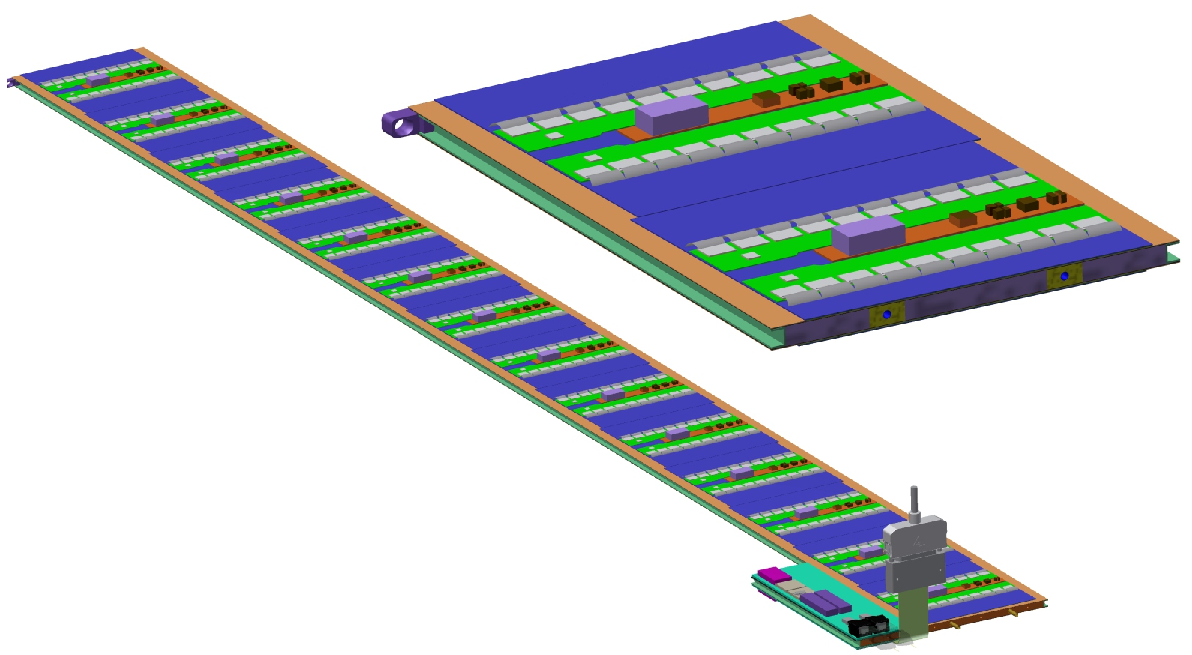
\includegraphics[width=0.8\linewidth]{figures/stave.pdf}
\caption{Strip barrel local support geometry. On the left, a complete stave is shown (EOS card in the foreground). The right picture shows a cross-section of the stave with the two cooling pipes visible inside the core. }
\label{fig:barrelgeometry}
\end{figure}

The endcap system consists of two endcaps composed of 6 disks each.
Each disk contains 32 `petals,' the local substructure depicted in Fig.~\ref{fig:endcapgeometry}.
Both sides of the petal are loaded with 6 modules, each with a distinct design,
located at increasing radius from the beam pipe and labelled R0 through R5 (where `R' stands for ring).
Each endcap module consists of one
or two wedge-shaped silicon sensors and a varying number of front-end chips and DC-DC converters.
% (between 12 and 28 ABCs, and 2 to 4 HCCs).
The EOS card is located adjacent to the R5 module, but the
cooling pipes run directly underneath it without a shared heat path, in contrast to the barrel EOS card.
Because of the unique geometry of each module in a petal, each of the six different types of module is
modelled separately in the thermo-electrical model.

\begin{figure}[ht]
\centering
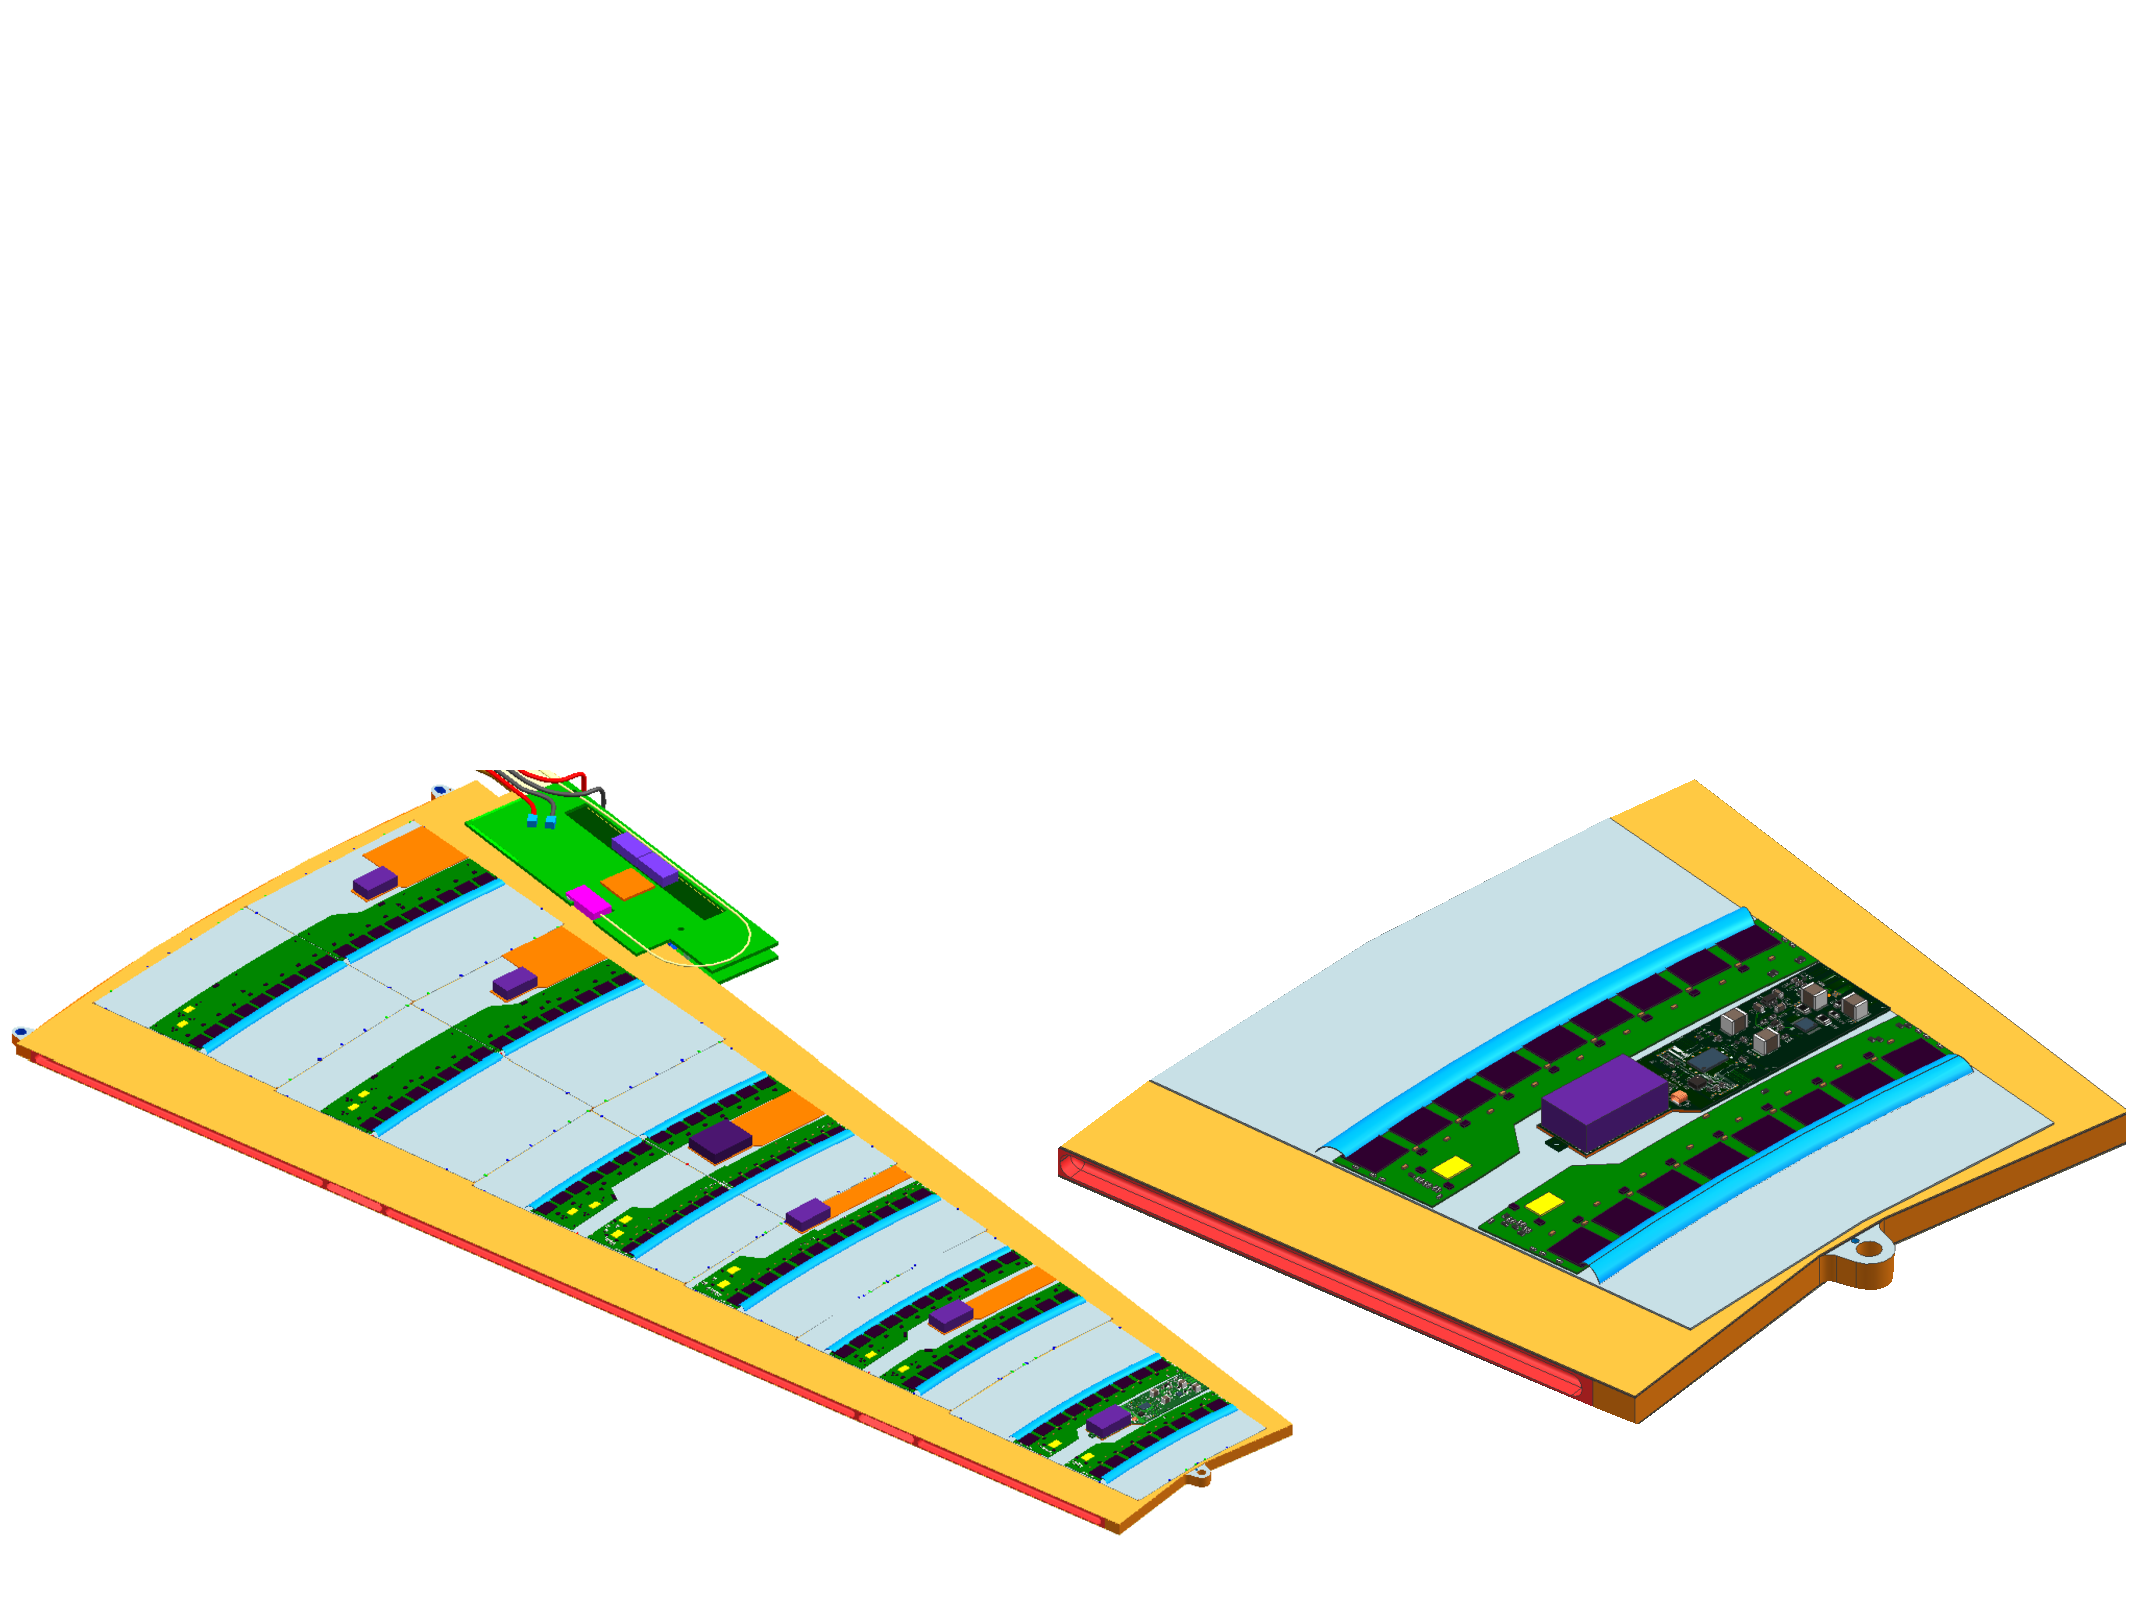
\includegraphics[width=0.8\linewidth]{figures/petal_and_closeup.pdf}
\caption{The geometry of the endcap strip petal, featuring 6 distinct module designs. A close-up of the R0 module is shown on the right.}
\label{fig:endcapgeometry}
\end{figure}

\subsection{Radiation environment}
A key input to the thermo-electrical calculation is the radiation environment of the strip system, as several inputs depend on radiation damage effects. The sensor leakage current can be parametrized as  a function of the fluence expressed in 1~MeV neutron-equivalents, and the TID effect on the digital chip current will be described as a function of the total ionizing dose rate (more details on its dependencies can be found in Section~\ref{fig:feast_eff}). 
% Change to ``non-ionizing energy loss (NIEL) fluence expressed in 1 MeV neutron-equivalents'' ??

Predictions for both of these quantities have been generated for each point in the ITk using the FLUKA particle transport code and the PYTHIA8 event generator (Fig.~\ref{fig:radiation}) \cite{background}. In the barrel system, both of these distributions display a strong dependence on $r$ but a weak $z$-dependence. Accordingly, we make the simplifying assumption that modules within the same barrel layer have identical fluence and TID, and model four different radiation profiles (one for each barrel layer). In the endcaps, the radiation levels vary significantly over the length of the petals and from disk to disk; therefore, we model each disk and ring position separately (36 in total).
% Note here: the fluence is a justification for modelling layer 0-3 separately, and using
% the flux/TID to model 6 separate versions of a petal.
% The module design justifies 2 (6) different module types in the barrel (endcap).

\begin{figure}[ht]
\centering
\subfloat[] {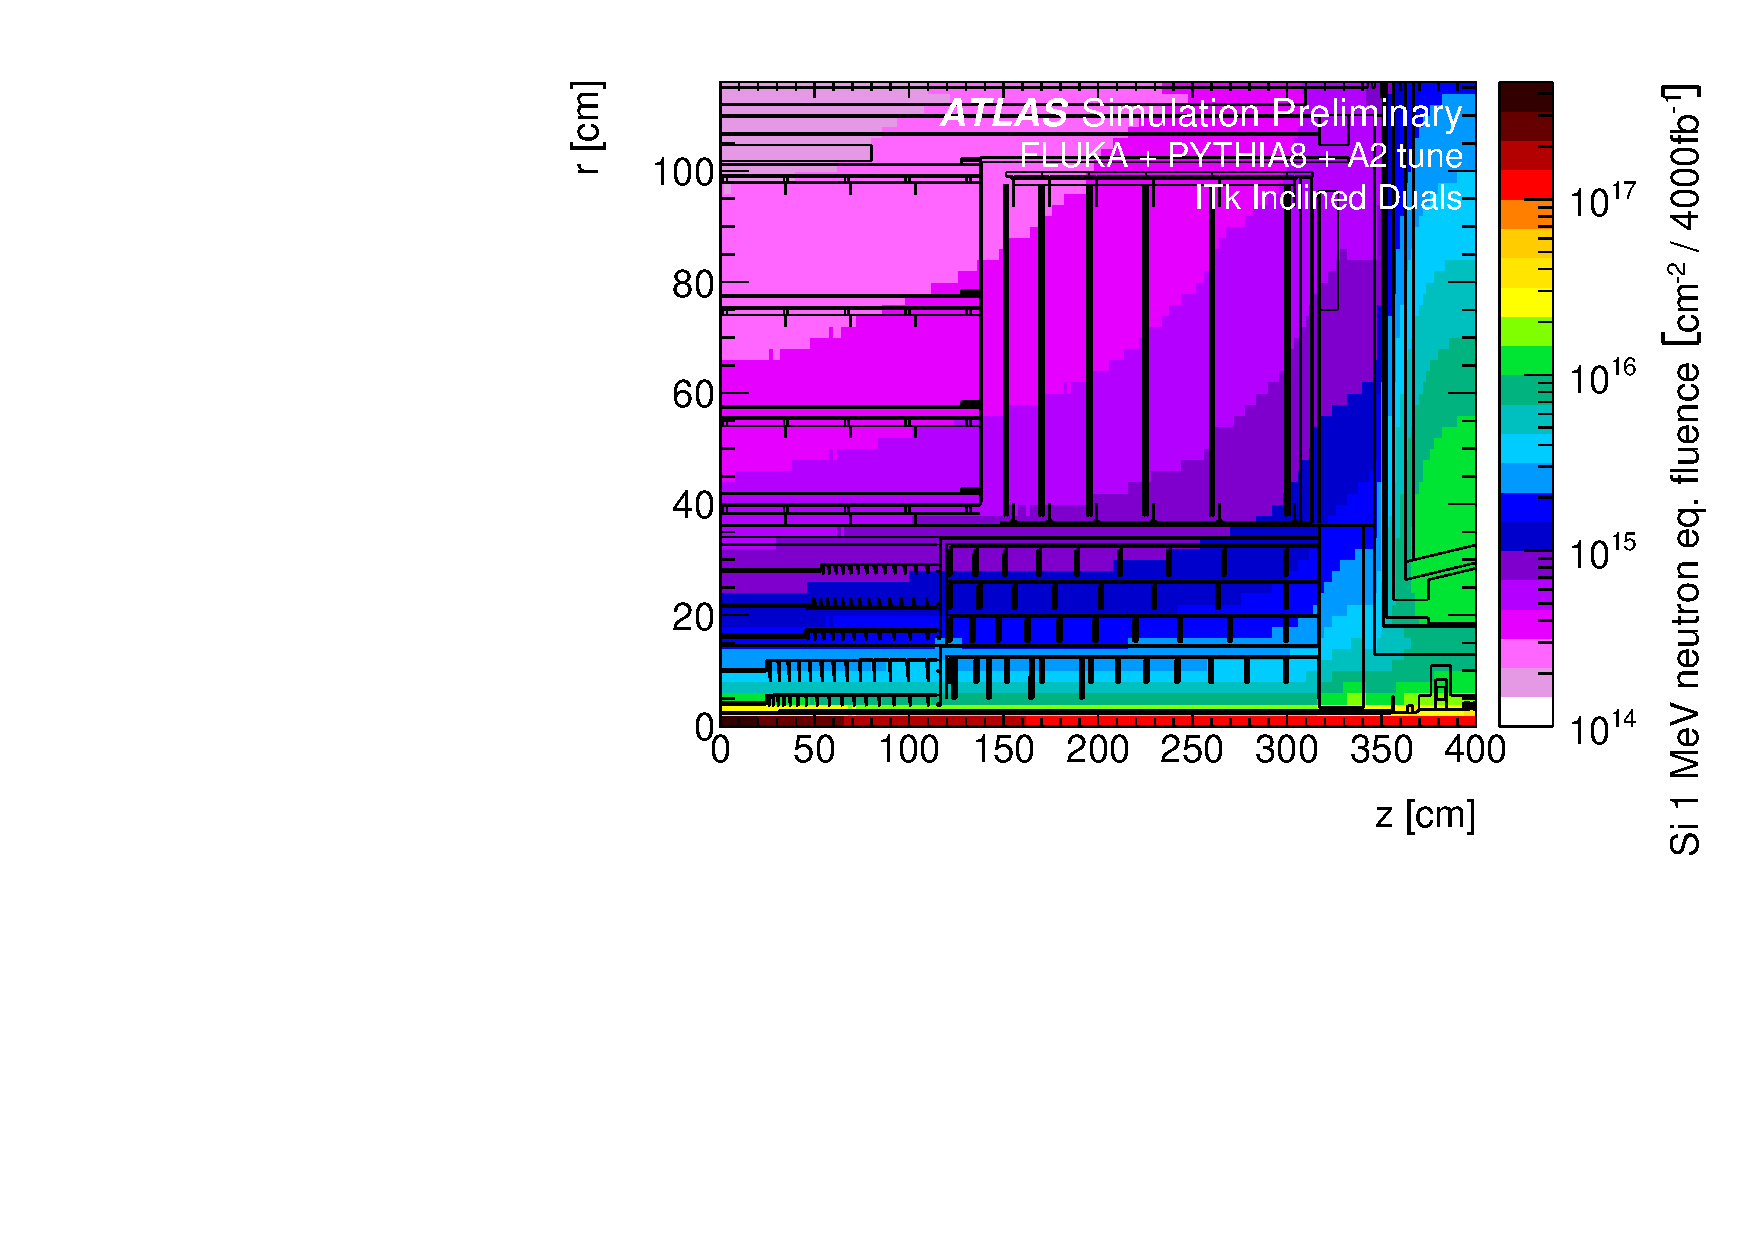
\includegraphics[width=0.48\linewidth]{figures/fluence.pdf}}\quad
\subfloat[] {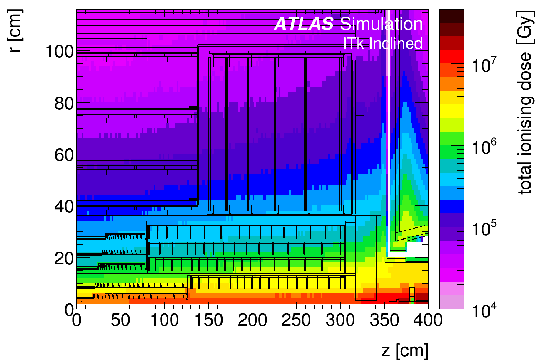
\includegraphics[width=0.48\linewidth]{figures/TID.pdf}}
\caption{The ATLAS ITk radiation environment. (a) 1~MeV neutron equivalent fluence and (b) total ionizing dose. Both plots are for an integrated luminosity of 4000~fb$^{-1}$ \cite{background}.
The figures use a rainbow colour gradient, with violet indicating the lowest values and red the highest values of fluence or ionizing dose.
}
\label{fig:radiation}
\end{figure}


\section{The electrical model}

The electrical model consists of low-voltage (LV) and high-voltage (HV) circuits, depicted in
Fig.~\ref{electrical_model}. The LV current (supplied at 11~V) is used to power the hybrid controller chips (HCCs) \cite{Collaboration:2017mtb},
ATLAS Binary Chips (ABCs) \cite{abc130} and Autonomous Monitoring and Control chip (AMAC) located on PCBs that are
glued directly onto the surface of the sensor.
These chips require between 1.5 and 3.3~V, which are provided by the temperature-dependent
FEAST DC-DC converter\footnote{
In the final version of the ITk strip system the FEAST chip is meant to be replaced by a chip
with similar functionality and behaviour, called the bPOL12V chip; we use the term FEAST
throughout this paper.} and an LDO (low-dropout) regulator (labelled linPOL12V in Fig.~\ref{electrical_model}).
The number of chips and converters on each module vary according to the design of
each different module type (barrel short-strip and long-strip modules, and six different endcap
module designs).
A barrel or endcap module contains 10--28 ABC chips, 1--4 HCCs, and
1--2 of each of the other components (linPOL12V/FEAST/AMAC).

\begin{figure}[ht!]
\centering
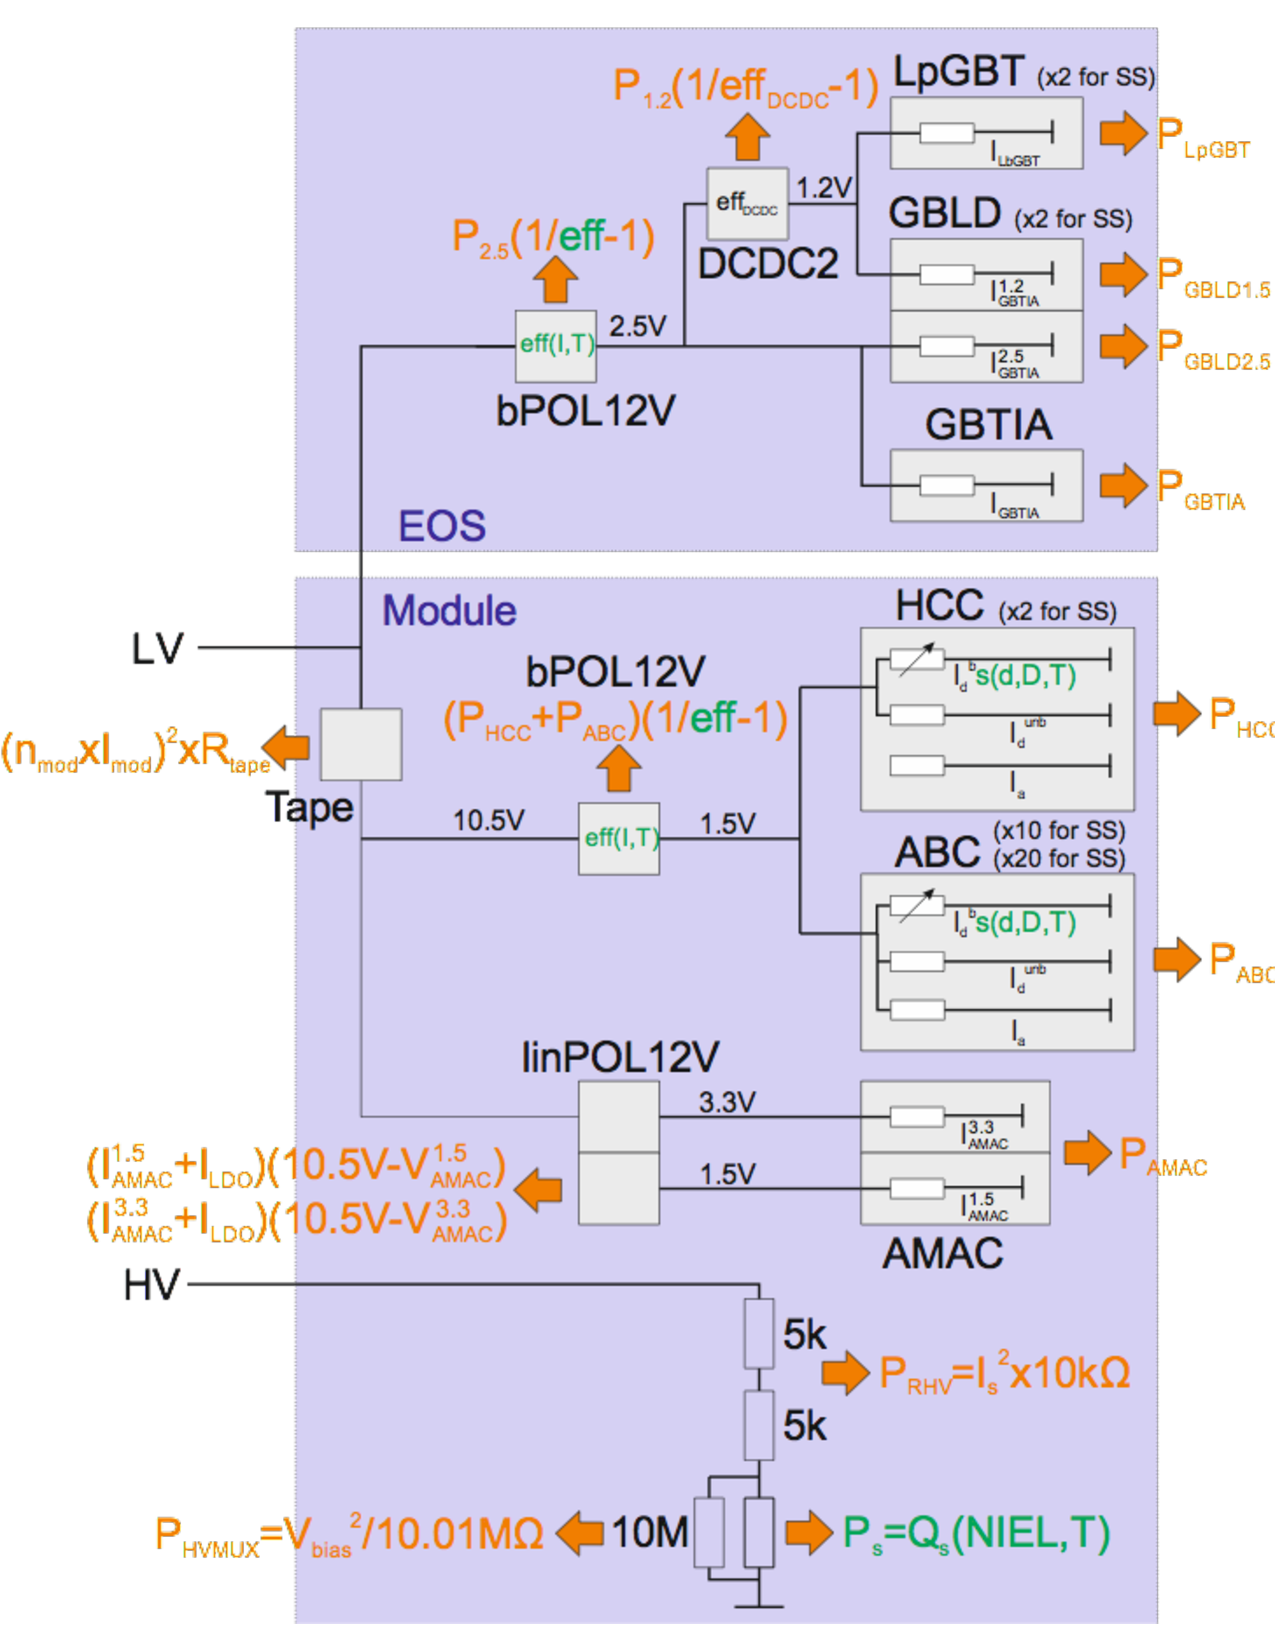
\includegraphics[width=0.8\linewidth]{figures/electrical_model.pdf}
\caption{
The electrical model of the ITk Strip barrel and endcap modules. Green arrows represent temperature-dependent heat sources, while orange arrows are temperature-independent. Grey squares are chips.
% Chip counts per module are linPOL12V/FEAST/AMAC: 1 each (2 each for EC R3); HCC: 1 for barrel LS, 2 for barrel SS and EC R0-R2 and R4-R5, 4 for EC R3; ABC: barrel: 10, 20 (LS, SS), EC: 17, 21, 21, 28, 16, 18 (R0-R5).
}
\label{electrical_model}
\end{figure}

%% The ABCs and HCCs are all powered at 1.5~V using a DC-DC converter (the FEAST) to step the voltage down
%% from 11~V (linPOL12V and FEAST in Fig.~\ref{electrical_model}). Typically one FEAST per module is used to power the chips; however, due to the large
%% number of ABCs on endcap module R3, the load is split across two FEAST converters on the module.

%% The AMAC contains a component powered at 1.5~V and one powered at 3~V; both are delivered from the
%% 11V source by an LDO regulator with a 1.9~mA quiescent current.
%% Again, the endcap module R3 differs from other modules, containing two AMACs each powered by its own
%% LDO.

The LV current is also delivered to the EOS card to power various data transfer components:
the Gigabit Laser Driver (GBLD), low power GigaBit Transceiver (LpGBT) and Gigabit Trans-impedance Amplifier (GBTIA) chips.
A FEAST identical to the one used on the module is used to step the
voltage down from 11~V to 2.5~V, and an additional DC-DC converter (`DCDC2') brings the voltage down further for some components.
%% The EOS cards on the endcap petals and the long-strip staves have one GBLD and one LpGBT;
%% EOS cards on the short-strip staves contain two of each. All EOS cards contain one GBTIA.
The short-strip barrel staves contain two GBLD and LpGBT chips.

The bus tape, which carries both LV and HV currents, has a small ohmic resistance, which impacts the
module in two ways. First,
the tape itself will generate some heat according to the amount of current passing through it; this
source of heat is accounted for in the model, however the contribution to the total module power
is negligible.
Second, due to the voltage loss along the traces, there is a slight reduction in voltage supplied to successive modules along the substructure.
The treatment of this effect is slightly different in the barrel and
endcap models: in the barrel, the voltage delivered to every module is averaged to 10.5~V; in the endcap,
the $\Delta V$ is estimated based on the calculated expected power loss along the tape for each module and varies between 10.8 and 11~V.
In both the barrel and endcap systems, the impact of using a different treatment is small.

Finally, the HV current provides the bias voltage on the silicon sensors. An HV multiplexer
switch (HVMUX) can be used to disconnect the sensor from the
bias line (it requires a 10~M$\Omega$ resistor parallel to the sensor in order to function). Two HV filters with an effective resistance of 10~k$\Omega$ are situated in series with the
sensor. The nominal operating voltage of the sensor is expected to be 500V, but the system is designed
to handle a bias voltage of up to 700V.


\section{The thermal model}
The thermal network consists of heat sources (some of which are temperature-dependent) and thermal resistances. The latter are given by the properties of the mechanical design (heat conductivities of the materials) and the geometry of the heat path. The geometry is generally 3-dimensional, but it is the strategy of the simple network models to lump the 3D behaviour into one thermal resistance parameter. In the models discussed here, we have used a granularity corresponding to single detector modules for which the thermal resistance has been modelled. The temperatures in the model are then given for the nodes in the network in analogy to the potentials in an electrical network.\footnote{Historically, Fourier's description of heat conduction pre-dated and inspired Ohm's work on electrical resistive networks. Here we followed the opposite direction.}

The complexity of the thermal network used in this study, depicted in Fig.~\ref{fig:thermalmodel}, is given by the variety of temperature-dependent heat sources in the ATLAS strip system. These sources consist of the digital power for each type of chip, the FEAST chip providing the on-detector DC-DC conversion, and the sensor leakage power. In the ATLAS ITk strip modules, all of these components are located on top of the sensors, such that the heat generated in them flows through the sensor into the support structure, the stave (barrel) or petal (endcap) core with the embedded cooling pipe. In the network model, the heat flow from these sources combines and travels through a common impedance $R_\text{M}$ to the sink at a temperature $T_\text{C}$. For each of the temperature-dependent heat sources (ABC, HCC, FEAST and the sensor) we have added a resistance from the common temperature $T_\text{mod}$ to allow for a finite and different heat path for each of them. Finally, the EOS card adjacent to the last module on the barrel stave or endcap petal is modeled as an additional source of heat with an independent impedance for its unique thermal path.

\begin{figure}[ht]
\centering
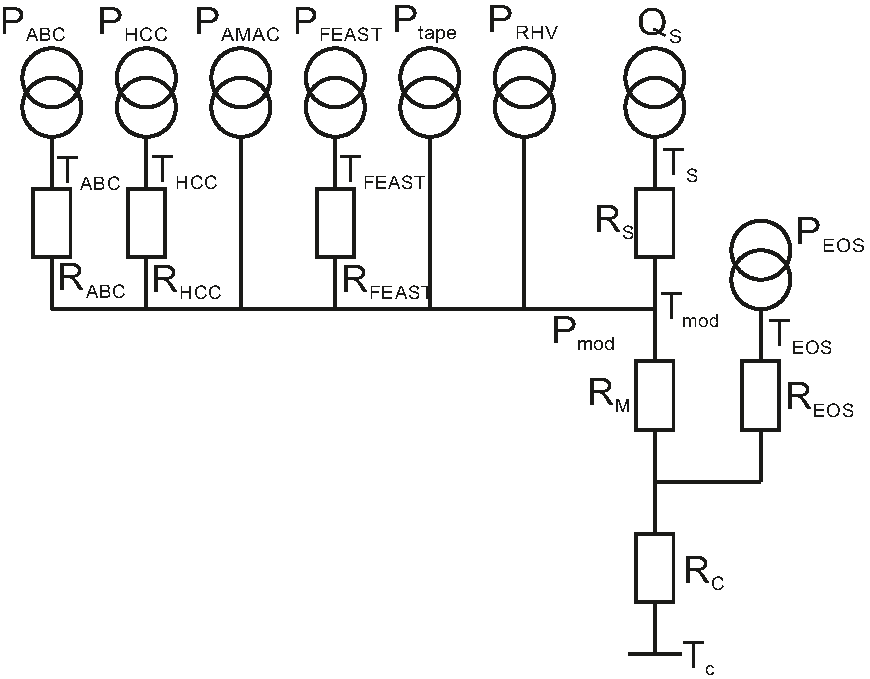
\includegraphics[width=0.6\linewidth]{figures/Thermalmodel.pdf}
\caption{Thermal network model.}
\label{fig:thermalmodel}
\end{figure}

This is a more complex thermal network than the one studied in Ref.~\cite{Beck:2010zzd}, for which an analytical solution for the determination of thermal stability is given. In particular, because of the non-linear temperature dependence of some of the heat sources, it is not possible in the present case to solve the set of equations describing the model analytically. However, the set of equations is still sufficiently small to solve numerically using functional programming languages such as Mathematica (used in the barrel model) or Python (used in the endcap system).


\section{Obtaining thermal impedances using FEA}
\label{sec:impedances}

The cooling path between the sources dissipating electrical power and the cooling fluid is 3-dimensional and includes components with orthotropic thermal conductivity. Hence the prediction of temperature at any node of the model requires a 3D thermal FEA \cite{abaqus,ansys}. However, the thermal conductivities of the components along the path are approximately constant, so that the temperature rise $\Delta T_i$ above the coolant temperature of any node $i$ ($i=$~ABC, HCC, AMAC, FEAST, tape, RHV, or sensor) in the thermal network model is adequately described by a linear sum of contributions from individual sources, i.e:

\begin{equation}
\Delta T_i \equiv T_i - T_C = R_i P_i + \left(R_\text{C} + R_\text{M}\right)\sum_j P_j,
\label{eq:deltaT_expression}
\end{equation}
where the index $j$ runs over all powered nodes. (We have momentarily ignored the contribution from the EOS card.)

In order to extract the thermal impedances for the thermal network model, the finite element model is run multiple times, with each heat source (or group of similar sources) switched on in turn with a representative amount of heat. In each of these cases, the temperature is calculated for all nodes in the thermal network model (Figure~\ref{fig:thermalmodel}). The temperature of a node is here taken as the average of the temperatures for all the gridpoints in the FEA model within the volume of the object corresponding to the node\footnote{This is particularly interesting in the case of the sensor, which fills a large volume, with a potentially large range of temperatures. In Ref.~\cite{Beck:2010zzd} the analytic model parameters were extracted from the maximum sensor temperature predicted by FEA, whereas our subsequent studies have shown that the thermal stability limit is predicted more accurately if the average sensor temperature is used.}. The thermal impedances are then obtained from a fit of Eq.~\ref{eq:deltaT_expression} using the temperature data for all nodes for all cases of heat injection.

Because of the nature of the network, the fitted value for the common impedance $R_\text{CM}=R_\text{C} + R_\text{M}$ is determined by the observed temperature rises of components where no heat is injected. The linearity of this relationship is illustrated in Fig.~\ref{fig:solving_for_Rcm}. The value of each component-specific impedance is determined from the temperature rise observed when heat is injected into that component.

%The cooling path between the sources dissipating electrical power and the cooling fluid is three-dimensional and includes components with orthotropic thermal conductivity. Hence the prediction of temperature at any node of the model requires a 3d thermal FEA Ref [Abaqus, Ansys]. However, the thermal conductivities of the components along the path are approximately constant, so that the temperature rise (above Tc) at any node of the structure is adequately described by a linear sum of contributions from individual sources, i.e:
%\begin{equation}
%T_i  =   T_\text{c}  +  \sum_{j} a_{ij} Q_{j},
%\end{equation}

%(or group of similar sources) switched on in turn with a representative amount of heat, and the temperature rise noted for each of the nodes of interest, which are those in the thermal network model (Figure~\ref{fig:thermalmodel}).  

%BEGIN ALTERNATE DESCRIPTION
%Ignoring the EOS components momentarily, the temperature rise $\Delta T_i \equiv T_i - T_c$ of a given node $i$ can be expressed as:
%\begin{equation}
%\Delta T_i = R_i P_i + \left(R_{C} + R_{M}\right)\sum_j P_j\,, \quad i,j=(\text{ABC},\text{HCC},\text{AMAC},\text{FEAST},\text{tape},\text{RHV},\text{sensor}),/
%\label{eq:deltaT_expression}
%\end{equation}
%where the powered components are represented by the index $j$.
%In order to extract the coefficients $R_{i}$, $R_{C}$ and $R_{M}$,
%the finite element model is run multiple times, with each heat source (or group of similar sources)
%switched on in turn with a representative amount of heat, and the temperature rise
%noted for each of the nodes of interest, which are those in the thermal network model (Figure~\ref{fig:thermalmodel}).
%
%Using this data from the FEA, the quantity $R_{CM}\equiv R_{C} + R_{M}$ is first solved by
%focusing on the set of measurements where the measured temperature node ($i$)
%is not associated to the powered component ($j$).
%In these cases, the relationship can be expressed as:
%\begin{equation}
%\Delta T_i = R_{CM} P_j,
%\end{equation}
%assuming that only one source $j$ is powered at a time.
%Each pair of values for delivered power and $\Delta T$ is plotted in Fig.~\ref{fig:solving_for_Rcm}.
%The data is fit to a function of the form $\Delta T = R_{CM} \times P$;
%the slope of the line corresponds to the thermal impedance $R_{CM}$.
%The remaining thermal impedances ($R_\text{FEAST}$, $R_\text{ABC}$, etc.) are calculated by
%subsituting $R_{CM}$ into the equations remaining from Eq.~\ref{eq:deltaT_expression}.
%The value $R_{EOS}$ is calculated using a simlar procedure.

\begin{figure}[ht]
\centering
\subfloat[Barrel short strip module] {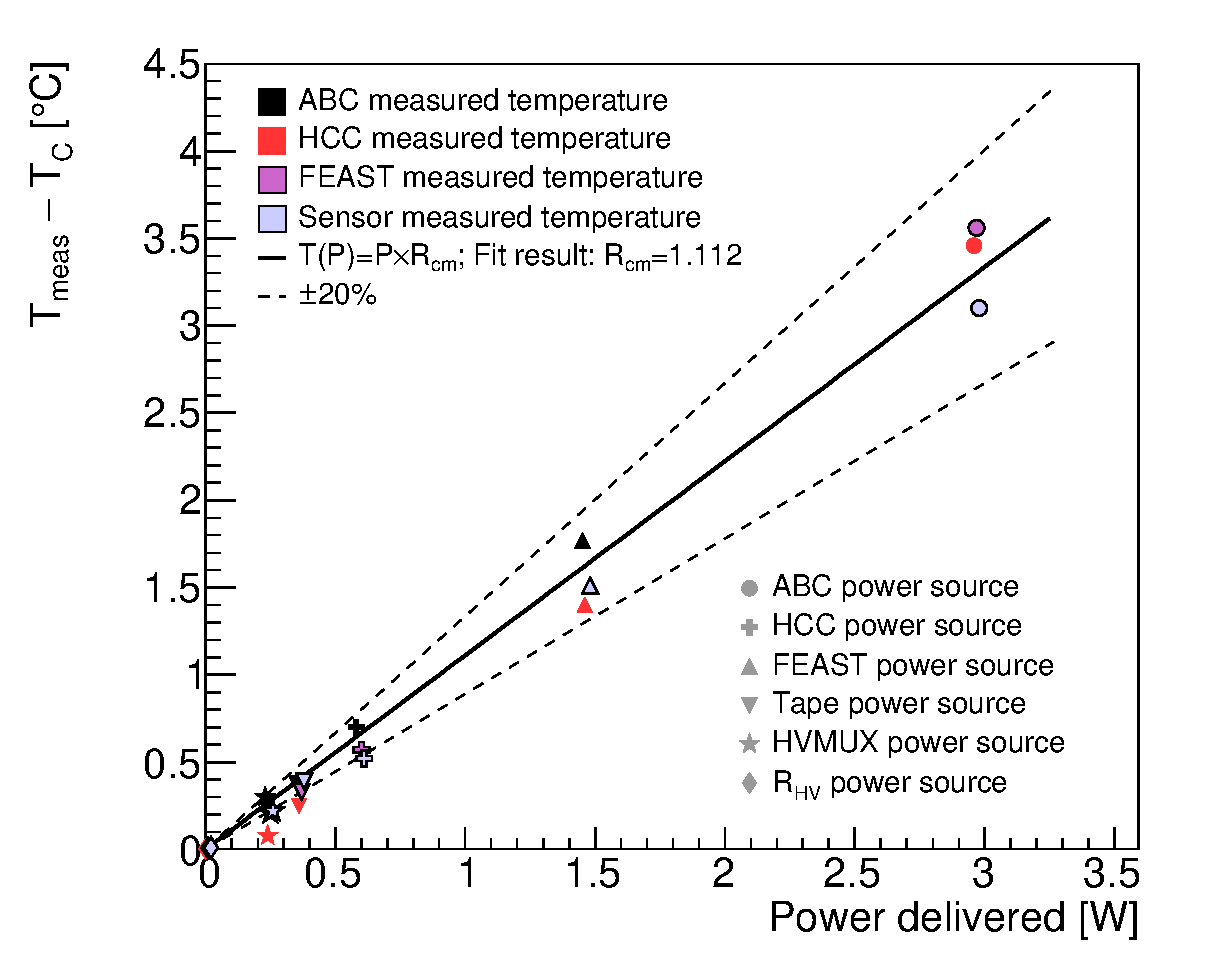
\includegraphics[width=0.45\linewidth]{figures/ThermalImpedanceFit_ShortStripEOS_Rcm.eps}}\quad\quad
\subfloat[Endcap R0 module] {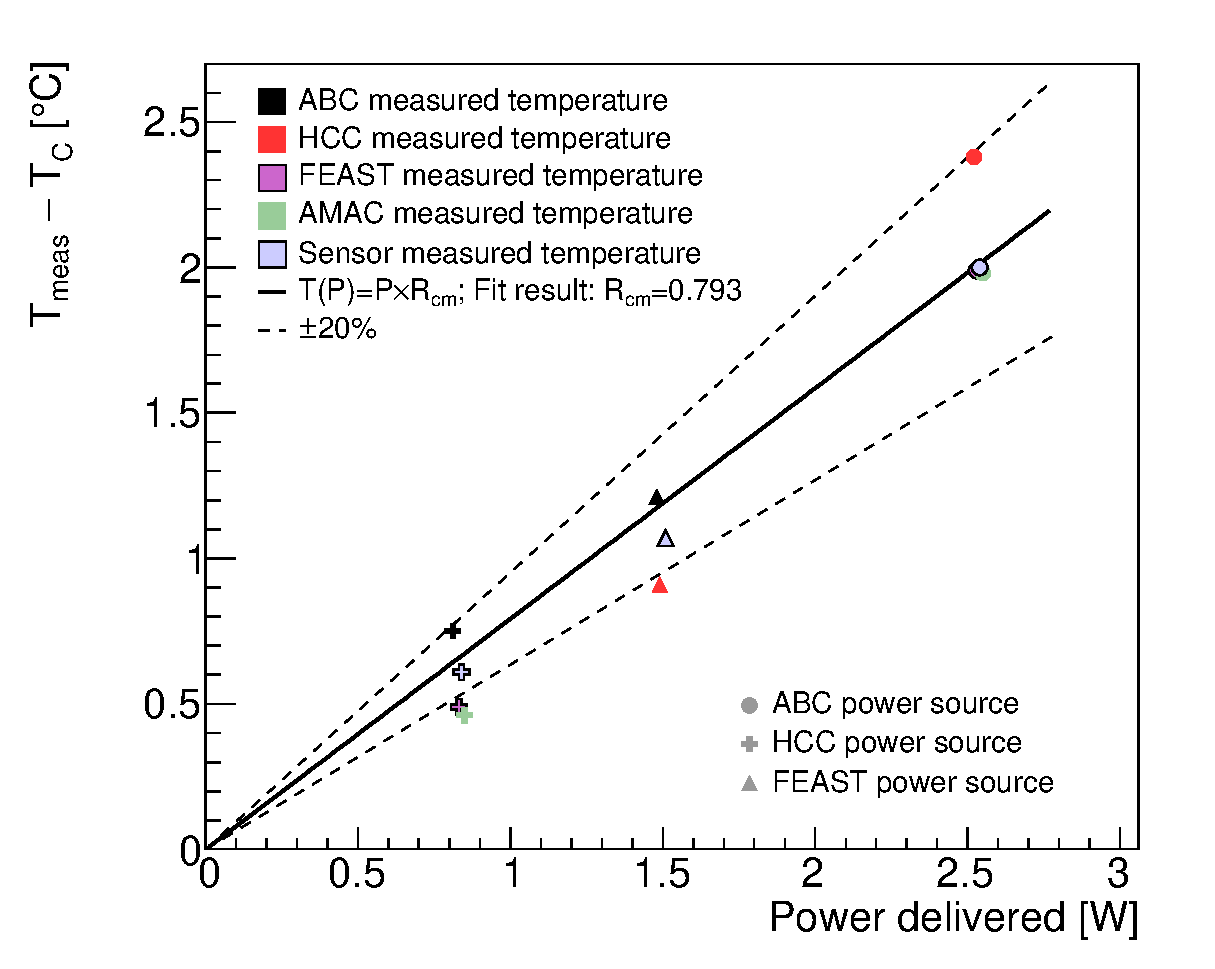
\includegraphics[width=0.45\linewidth]{figures/ThermalImpedanceFit_R0_Rcm.eps}}
\caption{The relationship between the temperature rise observed in the FEA for a specific component and the heat injected in another component. The slope of the fitted line is the estimate for $R_\text{CM}$.
(a) The fit for a short-strip barrel module adjacent to the EOS card. (b) The fit for the endcap R0 module.
For each data point marker, the source of power is indicated by the shape, and the measured component is indicated
by the color.
%% In (b), the error bars represent the standard deviation of temperatures of
%% that particular component, and are not considered in the fit.
The blue band represents a $\pm$20\% error band on the fit for $R_\text{CM}$.
}
\label{fig:solving_for_Rcm}
\end{figure}

%END ALTERNATE DESCRIPTION

For a barrel module, the agreement of the network temperatures using the thermal impedances from the fit with the data from FEA is better than 0.5$^\circ$C for all nodes. This procedure is performed for both an EOS module and a normal module. The thermal impedance from the sensor to the sink ($R_\text{CM}$) is consistently between 1.1 and 1.4~$^\circ$C/W, but higher values (between 10 and 20~$^\circ$C/W) are found for other impedances in the network ($R_\text{HCC}$ and $R_\text{FEAST}$), mostly because these are for components with a small footprint constituting a bottleneck for the heat flow.

% Endcap: 
For the endcap modules, the procedure to determine the thermal impedances is performed for
each of the 6 module types. $R_\text{CM}$ ranges from 0.6 to 1.4~$^\circ$C/W, with other nodes
between 5 and 20~$^\circ$C/W. Because the location of powered components is more irregular on an
endcap module, the difference between the predicted temperatures of the linear network and the FEA
can reach up to 1.2~$^\circ$C for key temperature-dependent nodes. To compensate for this additional
degree of uncertainty, the thermal impedance safety factor used in the endcap is increased by a factor of 2 compared to
the barrel modules (see Section~\ref{sec:safety_factors}).

There are two recognised departures from linearity of the thermal path: the rise in thermal conductivity of the silicon sensor with decreasing temperature, and the rise in heat transfer coefficient (HTC) of the evaporating CO$_2$ coolant with increasing thermal flux. The FEA models are run using mean values for these quantities appropriate to the operating conditions, and the thermo-electrical model results are insensitive to the variations expected in practice. However, if this level of realism is required and if reliable parametrizations for these dependencies can be obtained, then the inclusion of such variations in the model is possible.


\section{Other model inputs}

The two temperature-dependent elements of the thermoelectric model---the
radiation-induced digital current increase in the front-end chips, and the
efficiency of the FEAST DCDC converter---are described in this section.
Both effects are studied experimentally and fit with functional forms
in order to accurately represent them in the model.
The uncertainty in the experimental data, and in our modeling assumptions,
are estimated here and considered in the evaluation of safety factors,
described in detail in Section~\ref{sec:safety_factors}.

\subsubsection{DCDC converter}

The DCDC converter (FEAST) supplies a low-voltage (1.5~V) current to the ABC130 and HCC front-end
chips on the module.
The efficiency of the FEAST depends on its temperature as well as the output (load) current
load delivered to the front-end chips. To correctly model the FEAST efficiency, experimental
measurements are performed to characterize the dependence and fitted with a functional form.

To measure the FEAST efficiency, the FEAST power board was glued to an aluminum cold plate, cooled
with CO$_2$, and powered with the nominal working input and output voltages (11~V input, 1.5~V output).
The temperature of the FEAST was measured with an NTC thermistor and PTAT sensor residing on the FEAST,
for a range of load currents up to the maximum design current of 4A\footnote
{
FEAST data spreadsheet: \url{http://project-dcdc.web.cern.ch/project-dcdc/public/Documents/FEASTMod_Datasheet.pdf}.
Cite?
}.

The data was then fit with a function with sufficient parameters to ensure reasonable agreement; the
choice of functional form has no physical interpretation. Figure~\ref{fig:feast_eff} depicts the
FEAST efficiency data and the parameterized fit used in the model. The parameterization fits the data
with an acccuracy below 1\%; this unceratinty in the FEAST efficiency modeling is small
compared to other uncertainty sources, and is therefore neglected in our model.

\begin{figure}[ht]
\centering
\subfloat[] {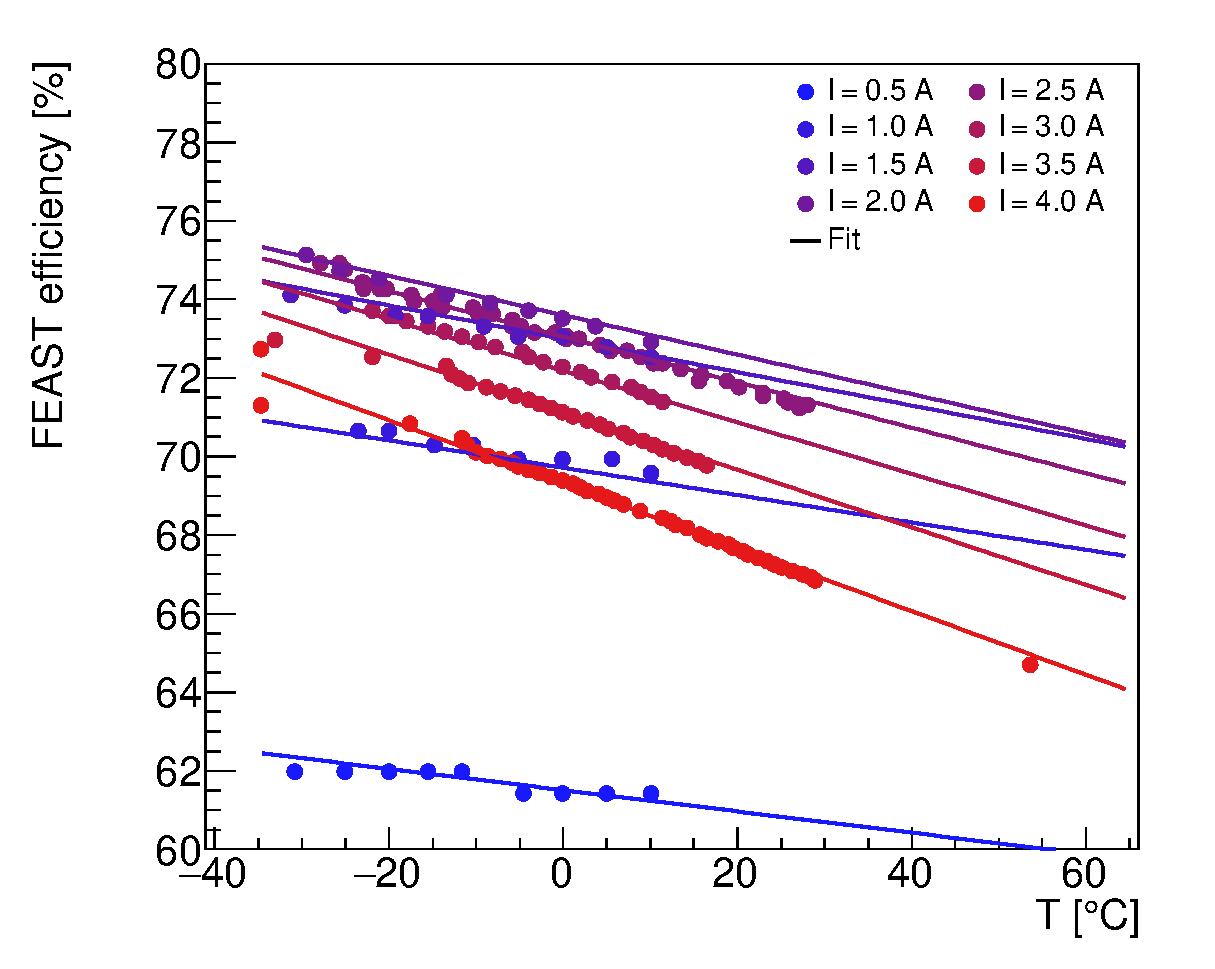
\includegraphics[width=0.49\linewidth]{figures/FeastEfficiency_isoCurrent.eps}}
\subfloat[] {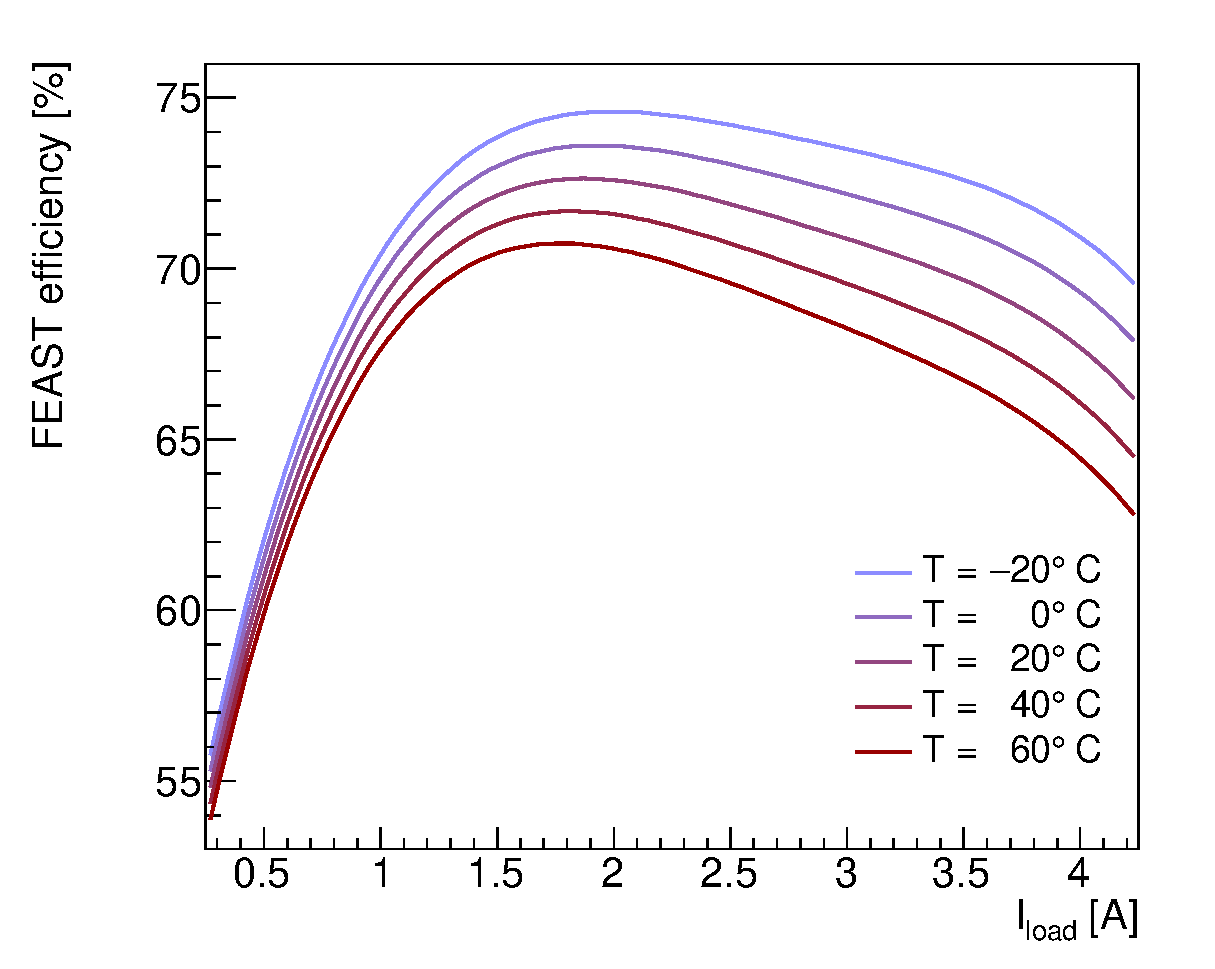
\includegraphics[width=0.49\linewidth]{figures/FeastEfficiency.eps}}
\caption{The FEAST efficiency model based on experimental data. (a) The experimental data points
characterizing the FEAST efficiency are plotted as dots and color coded for load current. The data is
compared to the analytic fit, evaluated in curves of equal current. (b) The same analytic fit,
presented as a function of current load for curves of equal temperature.
}
\label{fig:feast_eff}
\end{figure}


\subsubsection{Digital current increase of chips using 130~nm CMOS technology}
\label{sec:tid_explanation}

The ABC and HCC chips, designed using IBM 130 nm CMOS8RF technology, are known to suffer from an
increase in digital current when subjected to a high-radiation environment
\cite{Collaboration:2017mtb}. This phenomenon, known as the ``TID bump,'' is well-studied
\cite{1589217,FACCIO20081000} and has a characteristic shape whereby the effect reaches a maximum
over a period of time and then gradually diminishes (see Fig.~\ref{tid_bump}).

In an effort to characterize the nature of the TID bump in the ABC and HCC chips empirically,
many irradiation campaigns have been conducted using a variety of radiation sources, testing
the effect at different temperatures and dose rates.
The data collected from these studies was used to develop a model of the TID bump
that estimates the digital current increase given the total ionizing dose, the dose rate,
and the operating temperature of the chip. This parameterization, which is depicted in
Fig~\ref{tid_bump}, is used as an input to the thermoelectric model in order to correctly model the
ABC and HCC currents. The TID bump is assumed to fully apply to the HCC digital current, and apply to
69\% of the ABC digital current (according to our understanding of its digital circuitry).

\begin{figure}[ht]
\centering
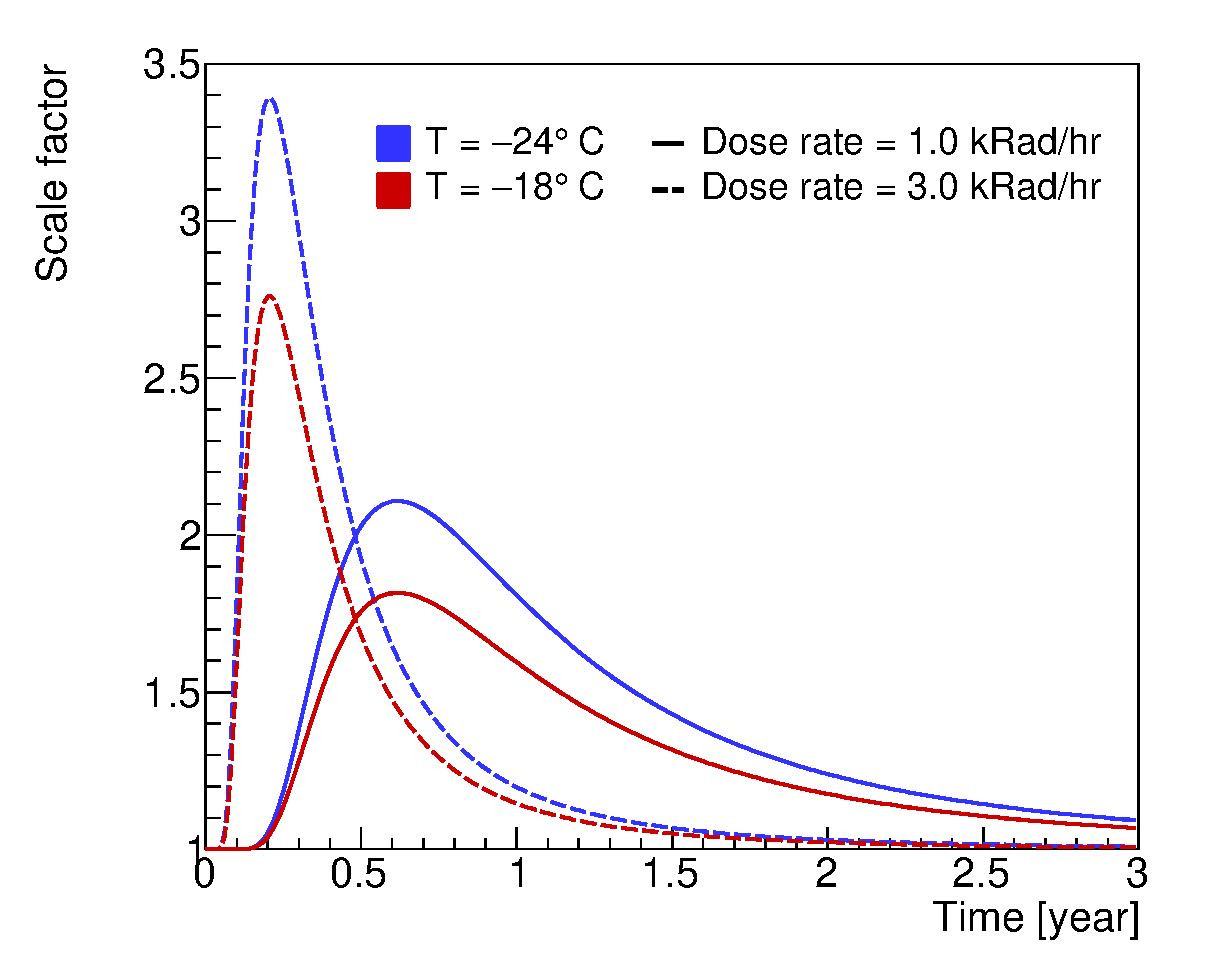
\includegraphics[width=0.5\linewidth]{figures/AbcTidBumpVersionRatesAndTemps_Nominal.eps}
\caption{Parameterization of the impact of the total ionizing dose
on the magnitude of the front-end chip digital current (the TID bump), presented as a function of time.
The current is multiplied by a scale factor that is modeled as a function of total ionizing dose,
dose rate, and temperature, based on experimental data.
}
\label{tid_bump}
\end{figure}

The TID bump displays certain key features, which are reflected in the parameterization:
first, the effect is larger at colder temperatures and higher dose rates. This means it can be
mitigated by operating the chips at higher temperature (note that the dose rate is fixed by the LHC conditions).
Second, the figure also illustrates how chips receiving different dose rates will reach their maximum
digital current increase at different times. This feature is particularly important when modeling the
total power consumed by the barrel and endcap systems. In both systems, the dose rate varies significantly
depending on the position of the module in the detector. The effect means that the maximum system
power will be smaller than the sum of the maximum power of each module, as each chip reaches
its maximum at a different point in time.

\subsubsection{Modeling flux and total ionizing dose in endcap modules}

Covered already in the introduction?



\section{Outputs of the thermal model}

\subsection{Operational scenarios}\label{sec:opscenarios}
To study the different aspects of our predictions for the operation of the ITk strip system throughout its lifetime we performed the calculation of the system parameters over the expected 14 years of operation in monthly steps. Time-dependent inputs to the calculations were given from the expected performance of the LHC (figure~\ref{fig:opscenarios}a) and different profiles for the cooling temperature. We studied flat cooling temperature scenarios at different temperatures starting at -35$^\circ$C, the lowest evaporation temperature achievable with the ITk evaporative CO$_2$ cooling system, and a `ramp' scenario, where the cooling temperature starts at 0$^\circ$C and gradually is lowered down to -35$^\circ$C (figure~\ref{fig:opscenarios}b).

\begin{figure}[ht]
\centering
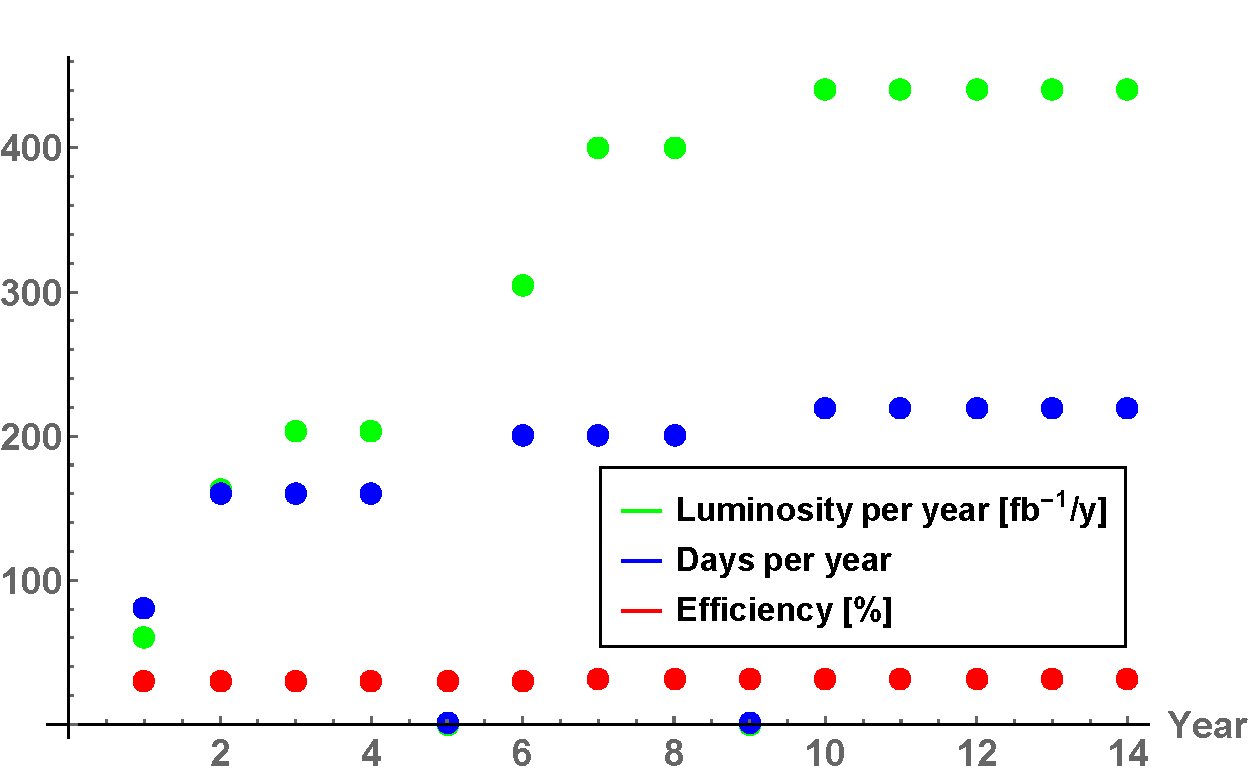
\includegraphics[width=0.4\linewidth]{figures/LHCperformance.pdf}\quad\quad
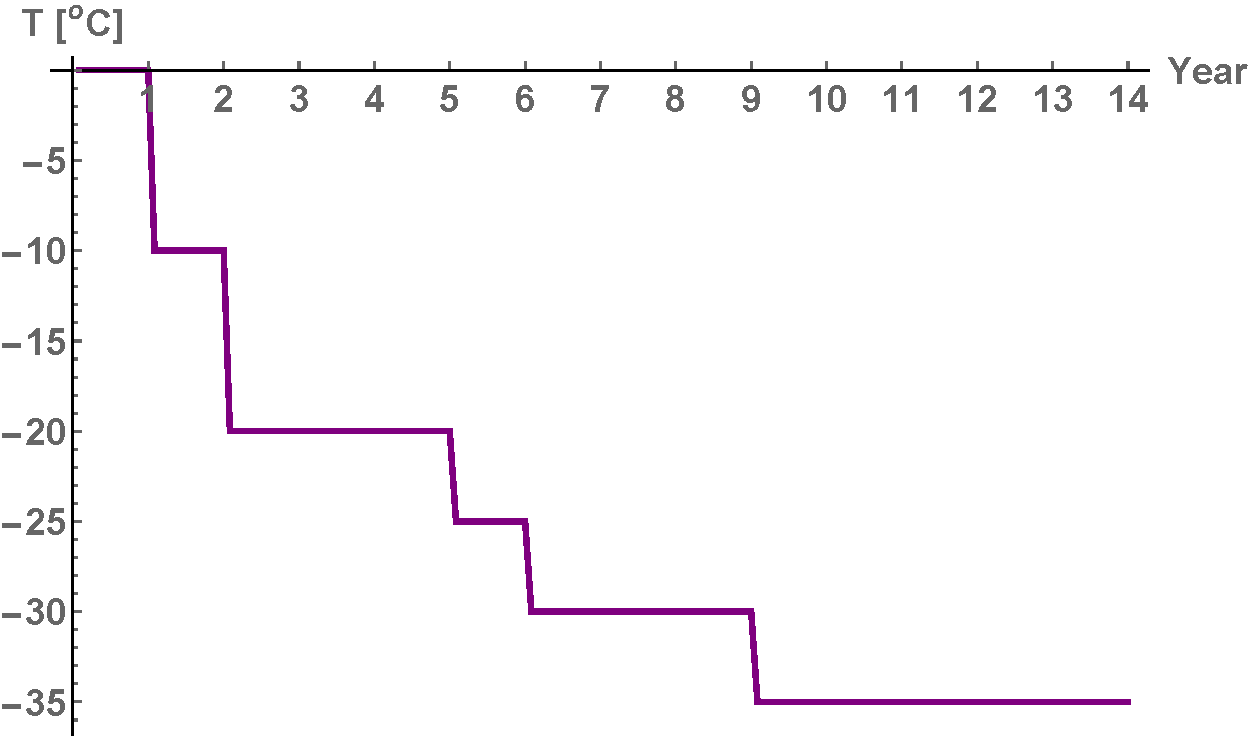
\includegraphics[width=0.4\linewidth]{figures/coolingramp.pdf}
\caption{Expected LHC performance (left) and cooling ramp' scenario for the cooling temperatures (right). Year-long shutdowns of the LHC are anticipated in years 5 and 9.}
\label{fig:opscenarios}
\end{figure}

\subsection{Safety factors}
To ensure the robustness of the system design against errors in the assumptions used in the model we ran the model in addition to the nominal set of input parameters with a set where some key inputs have been degraded. The set of safety factors used are given in table~\ref{tab:safetyfactors}. Each safety factor has been estimated individually based on experience, the complexity of the system aspect described by the parameter, and from available data or the absence of such data. Note that when the model was evaluated with safety factors all the safety factors in table~\ref{tab:safetyfactors} were used together, a situation which is unlikely to occur in the real system, thus providing a worst case estimate for the performance of the ITk strip system.

\begin{table}[htb]
\caption{Safety factors.}
\label{tab:safetyfactors}
\centering
\begin{tabular}{lcl}
Safety factor on & Value & Reason \\
\hline
Fluence  & 50\% & Accuracy of fluence calculations and uncertainties in material distributions\\
Thermal impedance & 10\% & Local support build tolerances\\
Digital current & 20\% & Final chip performance and parametrization of TID effect\\
Analog current & 5\% & Final chip performance\\
Tape impedance & 10\% & Electrical tape manufacturing tolerances\\
Bias voltage & 700~V & Increased bias voltage from 500~V to maintain S/N\\
TID parametrization & Nominal/Pessimistic & Different data sets for fit of TID bump\\
\end{tabular}
\end{table}

\begin{figure}[ht]
\centering
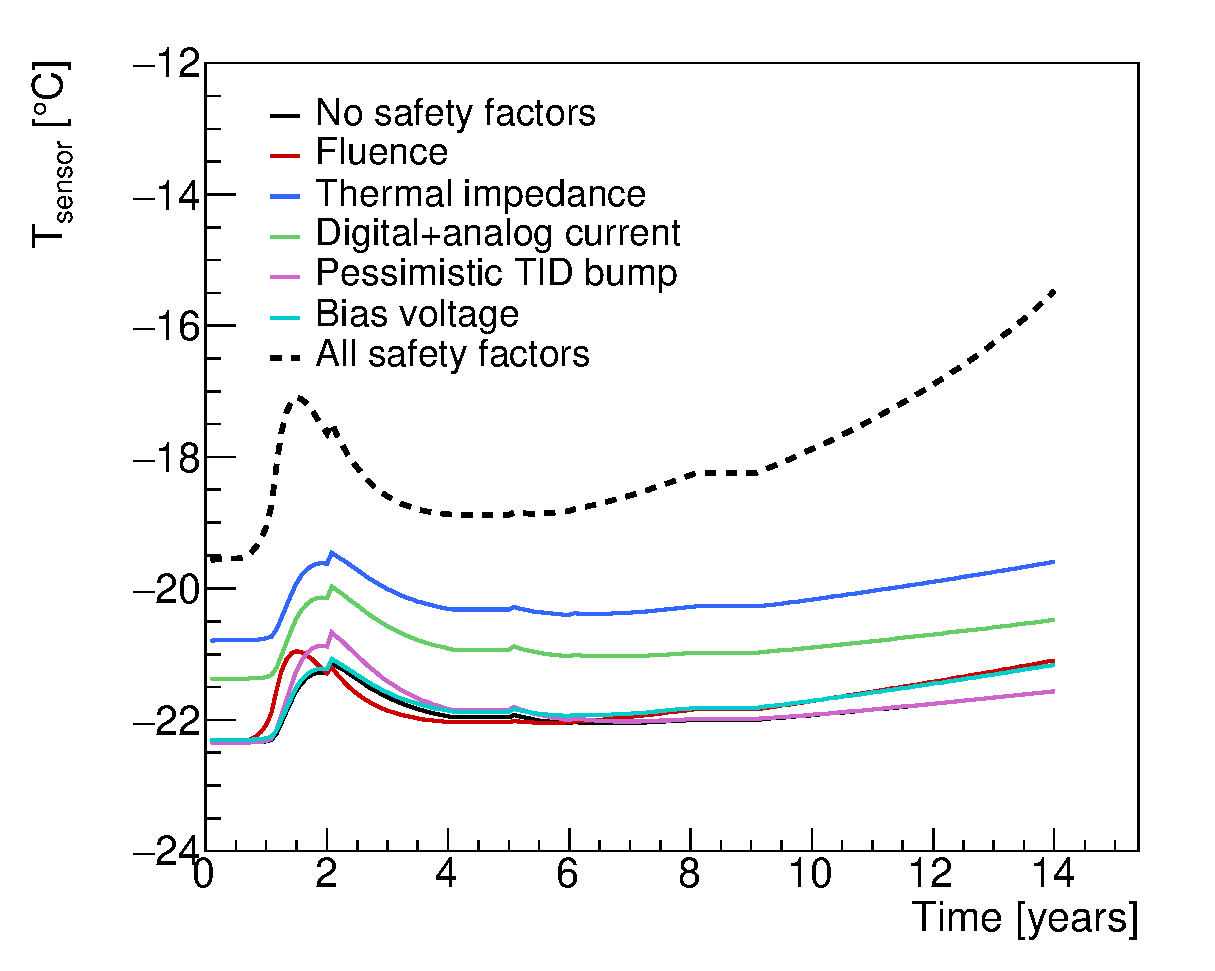
\includegraphics[width=0.49\linewidth]{figures/CompareSafetyFactors_SensorTemperature_R3.eps}
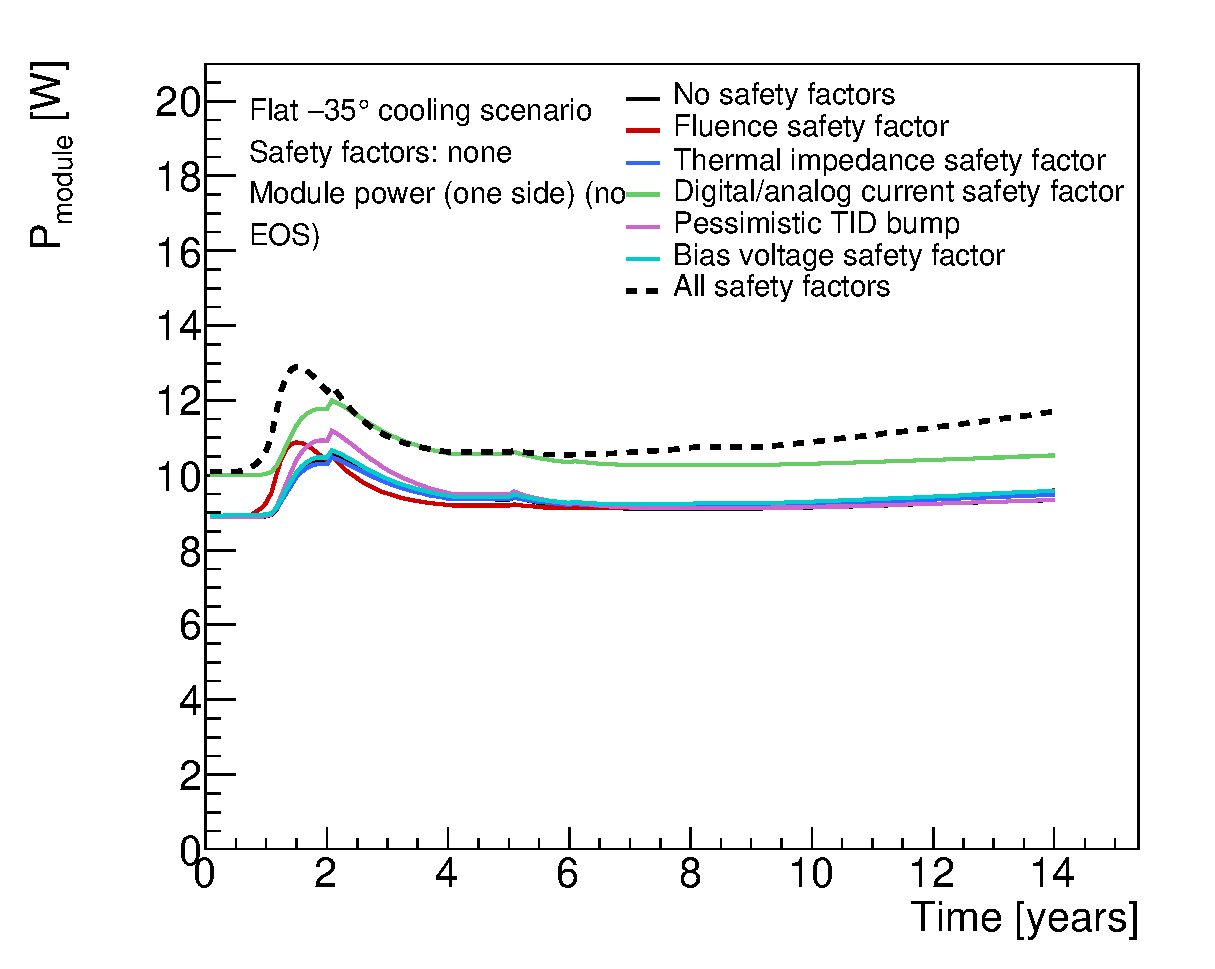
\includegraphics[width=0.49\linewidth]{figures/CompareSafetyFactors_ModulePower_R3.eps}
\caption{Comparing the impact of different safety factors.}
\label{fig:safety_factors}
\end{figure}

\subsection{Results}
The thermo-electrical model provides a large range of predictions for the operation of the strip system. A detailed discussion of all results would only be of interest for ITk strip community members and is beyond the scope of this article. Instead we will present here a subset of results to demonstrate the capabilities and use of the thermo-electrical model for the design of the detector system.

\subsubsection{Module properties}

Some example output plots for module properties from the thermo-electrical modules are shown in figures~\ref{fig:moduleflatperformance} and~\ref{fig:modulerampperformance}. The different radiation-dependent effects occur on different times scales. The maximum in the digital chip power due to the TID effect occurs relatively early (in year 1 to 4), although the bump has a long tail, particularly in the outer layers of the barrel. The sensor leakage power on the other hand grows towards the end of the lifetime of the ITk. Due to the radius-dependence of the radiation environment the radiation-induced effects are most pronounced in the innermost layer.

\begin{figure}[ht]
\centering
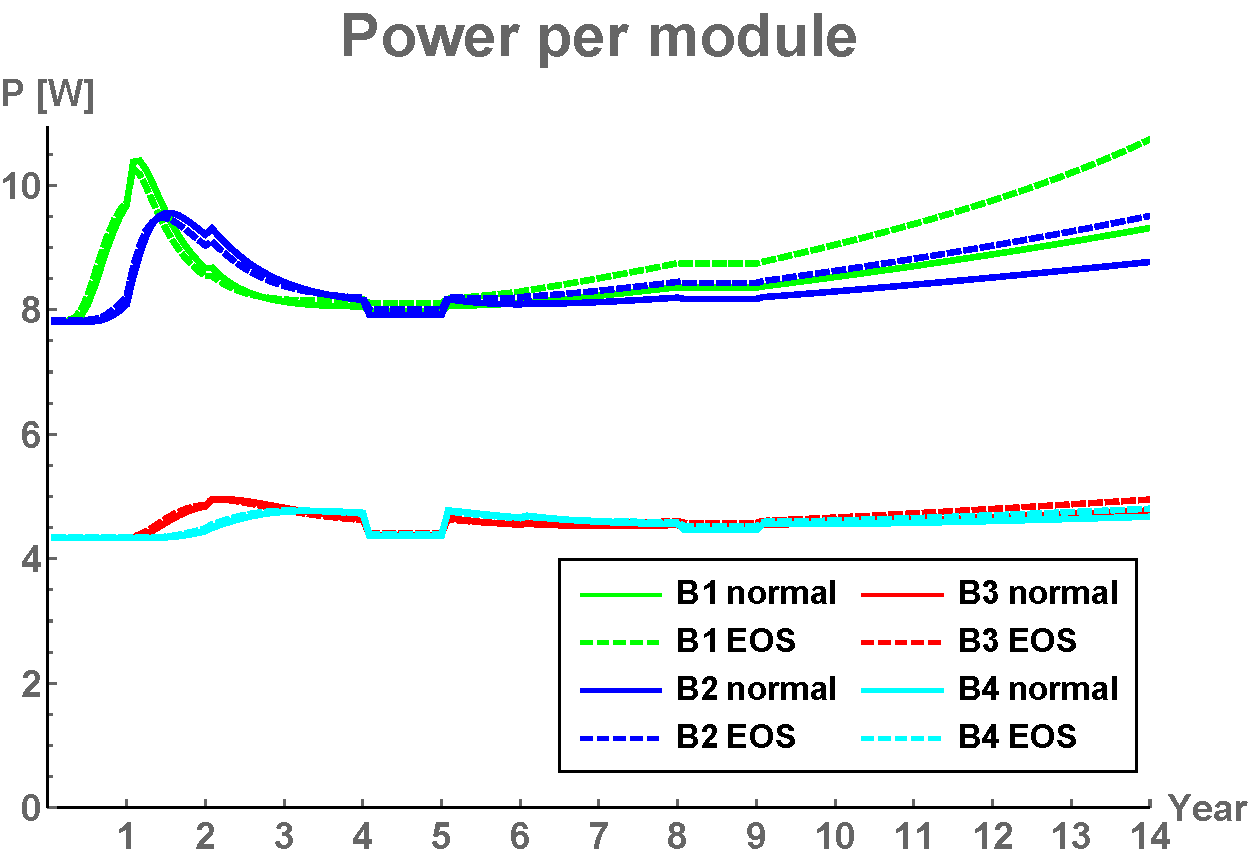
\includegraphics[width=0.4\linewidth]{figures/powerpermodule.pdf}\quad\quad
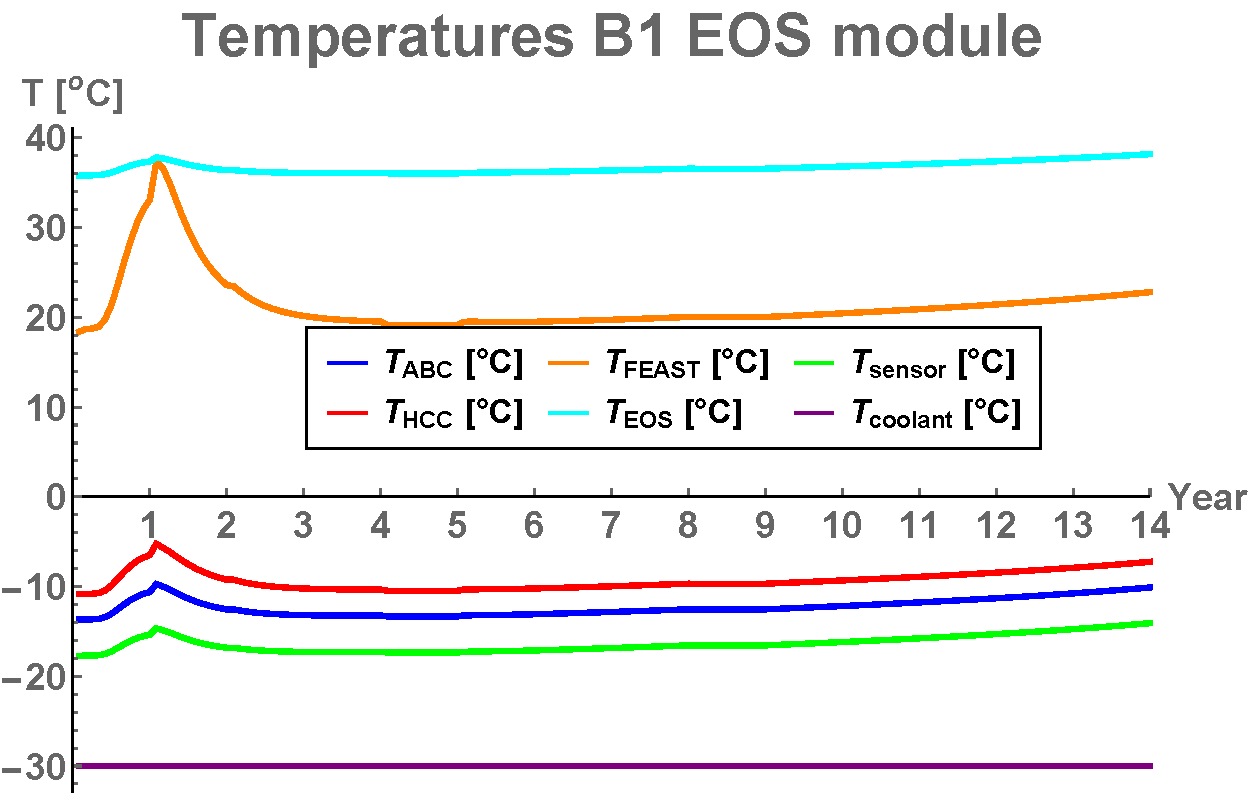
\includegraphics[width=0.4\linewidth]{figures/Teosmodule.pdf}
\caption{Examples for barrel module performance predictions for a flat cooling scenario (-30$^\circ$) including safety factors. Power per module (left). Temperatures for different parts of and end-of-stave barrel module in the innermost barrel (right).}
\label{fig:moduleflatperformance}
\end{figure}

\begin{figure}[ht]
\centering
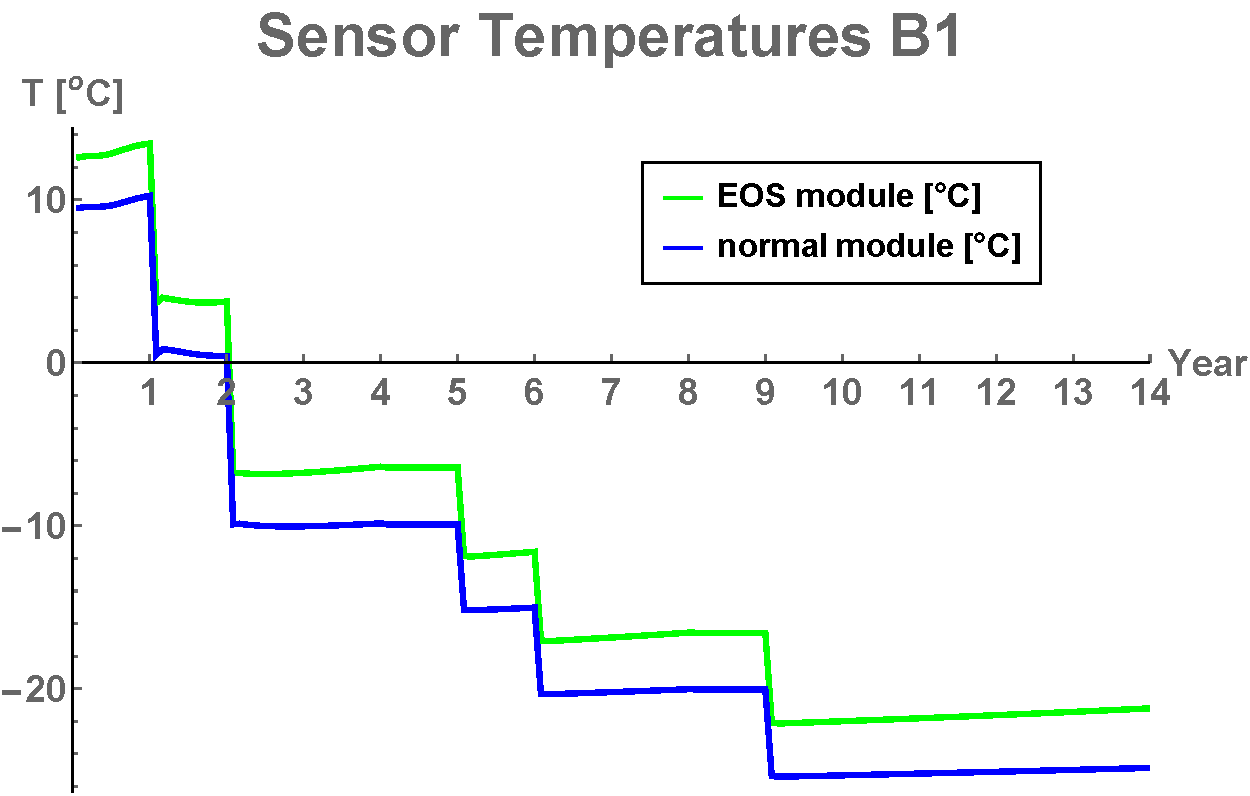
\includegraphics[width=0.4\linewidth]{figures/Tmodule.pdf}\quad\quad
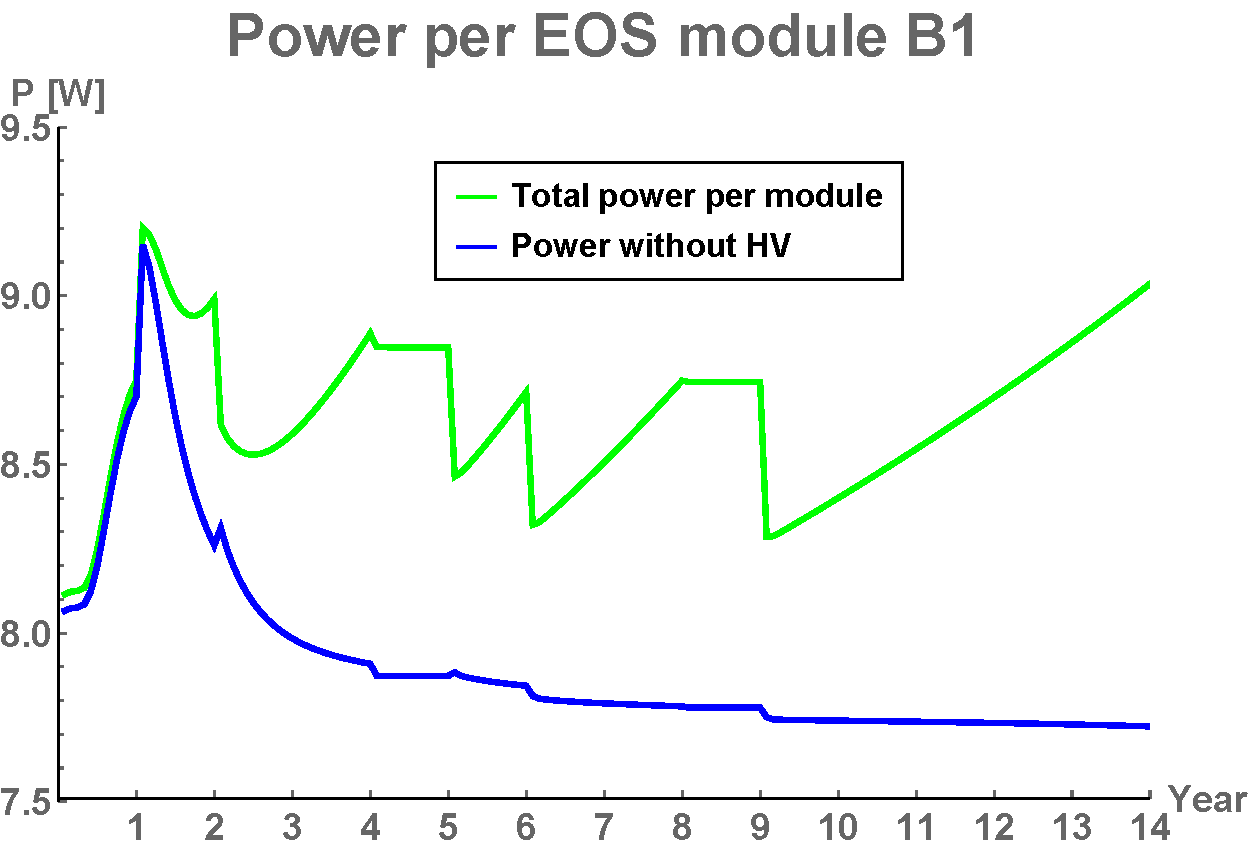
\includegraphics[width=0.4\linewidth]{figures/Peosmodule.pdf}
\caption{Examples for barrel module performance predictions for the ramp cooling scenario including safety factors. Temperature in innermost barrel modules (left). Power in an end-of-stave barrel module in the innermost barrel (right).}
\label{fig:modulerampperformance}
\end{figure}

\subsubsection{System properties}
One of the key concerns for the design of the strip system is thermal stability of the system. If the cooling temperature is too high to limit the leakage power from the radiation-damaged sensors to a level where it can still be removed the system is unstable (it goes into `thermal runaway'). In this case there is no solution to the set of equations in the thermo-electrical model any more and the numerical search for a solution fails. In the barrel strip system this happens in the last year of operation at a cooling temperature of -15$^\circ$C under nominal conditions, and at -25$^\circ$C (in year 13) with safety factors applied. As the design cooling temperature of the ITk cooling system is -35$^\circ$C we have confidence that the ITk strip system has sufficient margin for thermal stability.  

Beyond the issue of stability, the thermo-electrical model delivers predictions for the development of current and power requirements for the overall system. Some of the predictions are shown in figure~\ref{fig:systemperformance}. The Ignoring this time dependence could lead to overspecification of the cooling system.

\begin{figure}[ht]
\centering
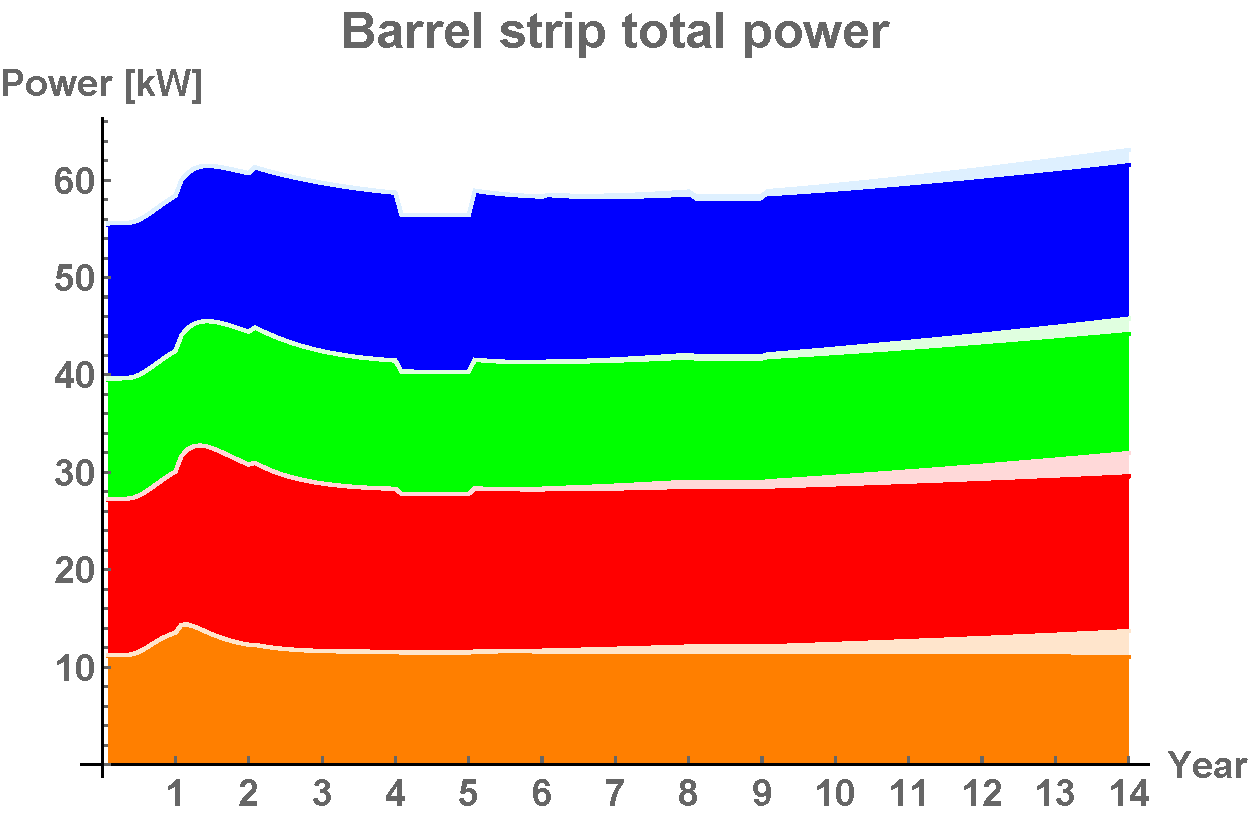
\includegraphics[width=0.4\linewidth]{figures/Totalbarrelpower-30.pdf}
\caption{Examples for system performance predictions. Barrel total power requirements for flat -30$^\circ$ cooling including safety factors (left): The plot shows the stacked power requirements for the four barrels (orange: innermost barrel, blue: outermost barrel). The greyed parts are contributions from HV power for the four barrels.}
\label{fig:systemperformance}
\end{figure}

These predictions are now used throughout the strip project to conistently size power supply and cooling systems. Including safety factors in the predictions gives us some confidence that the designs are robust and by using commonly agreed safety factors we ensure a consistent use of safety factors throughout the project and prevent safty factor creep.  

Because of the different timescales for the peak power due to the TID effect and the sensor leakage due to radiation there is room for the optimization of the cooling temperature profile for minimal power. The thermo-electrical model is a powerful tool to plan such an optimized cooling profile. In fact, the cooling `ramp' scenario introduced in section~\ref{sec:opscenarios} is the result of such an optimization (figure~\ref{fig:rampoptimization}).

\begin{figure}[ht]
\centering
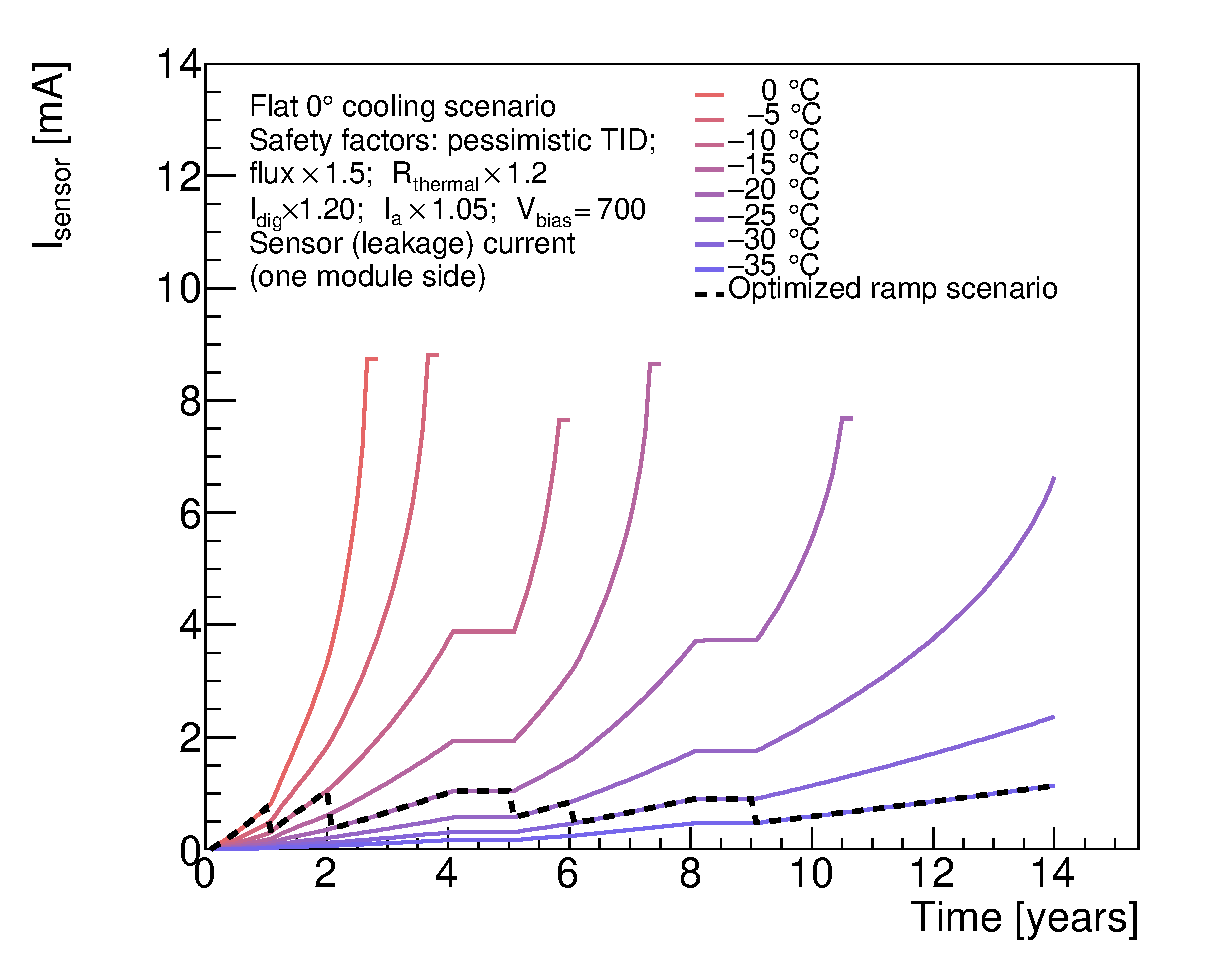
\includegraphics[width=0.49\linewidth]{figures/SensorCurrent_R3_newramp.eps}
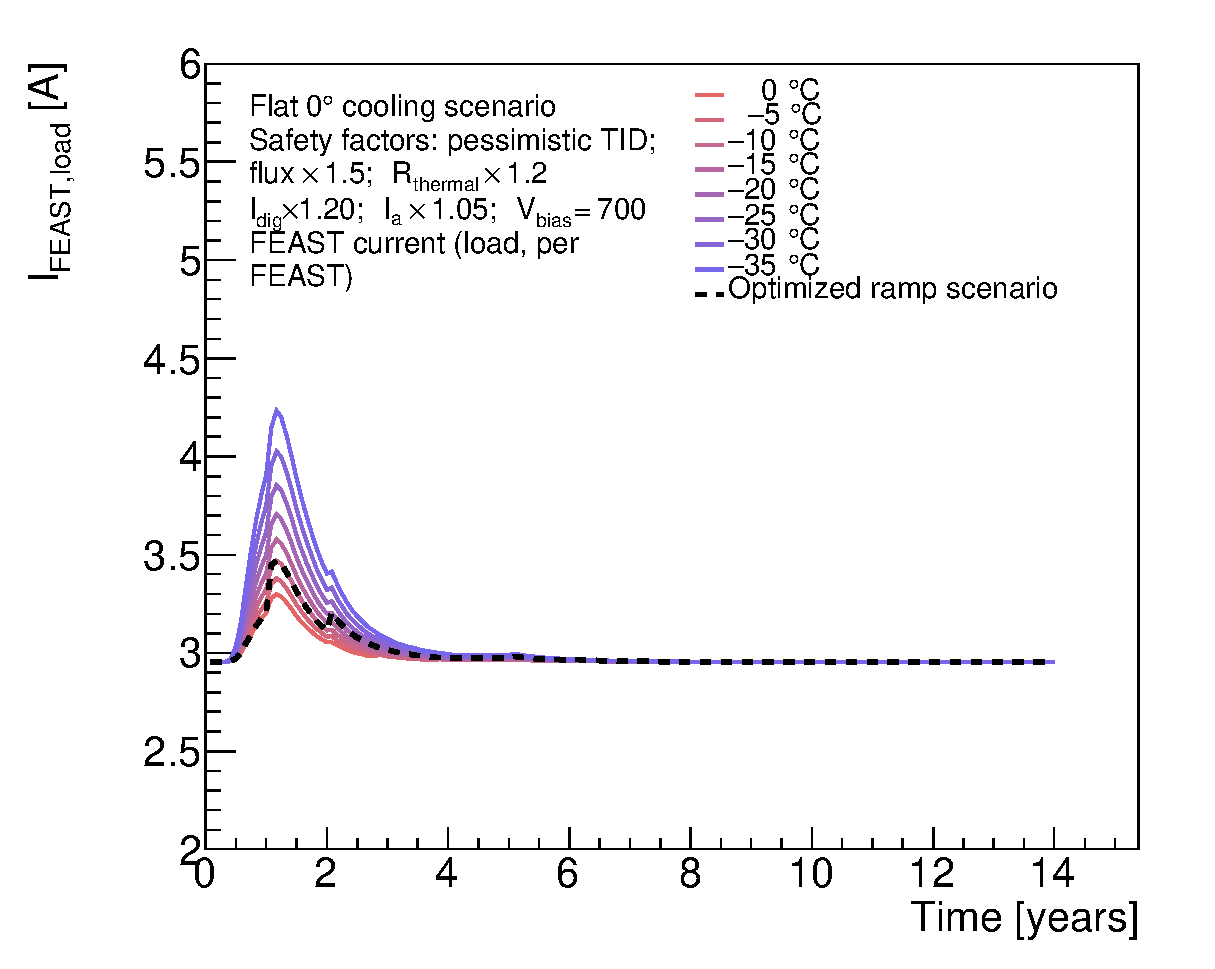
\includegraphics[width=0.49\linewidth]{figures/FeastCurrent_R1_newramp.eps}
\caption{Optimization of the cooling `ramp' scenario. The dashed lines represents the ramp scenario, which has been selected so that the sensor leakage current is stable throughout the lifetime of the ITk (left). The higher cooling temperatures in the first years keep the TID effect relatively small (right).}
\label{fig:rampoptimization}
\end{figure}


\section{Conclusions}
We have developed a model of the ATLAS ITk strip system that is based on the interplay between a thermal and an electrical network model. The set of equations in the model can be numerically solved using standard data analysis software in a short time, allowing for a quick turn-around for systematic studies of the system performance. The complexity of these networks is given by the number of interconnected components between the networks, many of which have a non-linear dependence on the temperature or electrical power. This approach can be easily adopted for any other silicon detector system.

In the case of the ATLAS strip system, several temperature-dependent heat sources had to be modeled. In addition to the sensor leakage current, these are the  radiation-induced increase of the digital front-end power (`TID bump') and the efficiency of the DC/DC conversion system. The outputs of the model give us confidence that the ITk strip system will be thermally stable until the end of LHC Phase-II operation, even with the inclusion of safety factors on key inputs. Furthermore, the model provides information for benchmark system parameters like cooling, supply power and currents in power cables, which is used in the specification of these systems. The use of the model outputs throughout the strip project ensures consistent specifications, including a common strategy on safety factors. Using the thermo-electrical model we can also propose an optimized cooling temperature `ramp' scenario, which equalizes leakage power throughout the lifetime of the experiment while minimizing the TID bump.

We have verified the performance of the thermal network model compared to a full FEA treatment, and we are confident that the level of disagreement is smaller than the uncertainty introduced by the model inputs. Among the inputs, the most likely source of unknown error stems from the limitations in our understanding of the parametrization of the TID effect.


\section{Acknowledgements}

(Acknowledgements.)


\bibliographystyle{elsarticle/elsarticle-num}
\bibliography{paper}

\end{document}
